% interactcadsample.tex
% v1.03 - April 2017

\documentclass[]{interact}

\usepackage{epstopdf}% To incorporate .eps illustrations using PDFLaTeX, etc.
\usepackage{subfigure}% Support for small, `sub' figures and tables
%\usepackage[nolists,tablesfirst]{endfloat}% To `separate' figures and tables from text if required
\usepackage{enumitem}
\usepackage{natbib}% Citation support using natbib.sty
\usepackage{amsmath}
\usepackage{multirow} 
\usepackage{algorithm}      
\usepackage{algorithmicx}   
\usepackage{algpseudocode}  
\usepackage{setspace}
\onehalfspacing  
\bibpunct[, ]{(}{)}{;}{a}{}{,}% Citation support using natbib.sty
\renewcommand\bibfont{\fontsize{10}{12}\selectfont}% Bibliography support using natbib.sty

\theoremstyle{plain}% Theorem-like structures provided by amsthm.sty
\newtheorem{theorem}{Theorem}[section]
\newtheorem{lemma}[theorem]{Lemma}
\newtheorem{corollary}[theorem]{Corollary}
\newtheorem{proposition}[theorem]{Proposition}

\theoremstyle{definition}
\newtheorem{definition}[theorem]{Definition}
\newtheorem{example}[theorem]{Example}

\theoremstyle{remark}
\newtheorem{remark}{Remark}
\newtheorem{notation}{Notation}
%\providecommand{\replace}[2]{#2} 
\begin{document}

\articletype{ARTICLE TEMPLATE}

\title{Two-stage attention-guided active learning for nonstationary Gaussian process modeling in robust parameter design}

\author{
	\name{Zebiao Feng\textsuperscript{a}\thanks{*Corresponding author. Email: zbfeng@njupt.edu.cn}, Xu Yang\textsuperscript{a}, Jianjun Wang\textsuperscript{b} and Weidong Huang\textsuperscript{a}}
	\affil{\textsuperscript{a}School of Management, Nanjing University of Posts and Telecommunications, Nanjing 210003, China;  \textsuperscript{b}Department of Management Science and Engineering, Nanjing University of Science and Technology, Nanjing 210094, China}
}

\maketitle

\begin{abstract}
Robust parameter design is vital for continuous quality improvement in industrial practice. However, modeling nonstationary response surfaces with limited data remains challenging because insufficient predictive accuracy may introduce optimistic bias in estimating the optimal parameter settings. We propose a two-stage attention-guided active learning method within a nonstationary Gaussian process (NSGP) modeling framework for robust parameter design. The method employs an acquisition strategy that integrates a softmax-weighted quality loss function with a maximin distance criterion to balance local accuracy around the potential optimum subregion and global space-filling. In the first stage, candidate design points are ranked by their relevance to the potential optimum subregion, and a high-weight subset is selected for further refinement. In the second stage, spatial diversity is enforced by selecting additional points from this subset to mitigate clustering. The selected points are then used to update the training set and the NSGP model. A genetic algorithm is employed to solve the NSGP-based robust parameter design problem and determine the optimal settings. Numerical experiments and engineering case studies show that the proposed method improves predictive accuracy and enhances the robustness of solutions in data-scarce scenarios.
\end{abstract}

\begin{keywords}
Quality engineering; robust parameter design; nonstationary Gaussian process modeling; active learning; two-stage attention-guided acquisition
\end{keywords}


\section{Introduction}
\subsection{Research motivation}
In modern manufacturing, product quality is directly linked to enterprise competitiveness, customer loyalty, and operational cost control, and is closely associated with improvements in market share and customer satisfaction \citep{Wu2011, He2021, Liw2025}. Systematic quality improvement further reduces defects, rework, and warranty expenditures \citep{Wu2020}. As a key approach in quality engineering, robust parameter design (RPD) determines the combination of design and process parameters to reduce sensitivity to noise factors, thereby enhancing the consistency and stability of quality characteristics \citep{Bao2016, Ouyang2016, Ouyang2025}. RPD has been widely applied in advanced manufacturing, engineering systems, and service operations, providing theoretical support for performance optimization under uncertainty \citep{Chuang2017, An2020, Huang2022}. Response surface methodology (RSM) is an important tool for implementing RPD by statistically approximating input–output relationships \citep{Fan2000, Ding2004, Peterson2009, Li2025}. However, the quality characteristics of modern engineering systems increasingly exhibit high dimensionality, strong nonlinearity, and pronounced nonstationarity. Under such conditions, conventional response-surface or surrogate models struggle to achieve adequate accuracy and generalization with limited data. This limitation undermines both the validity of optimal solutions and the efficiency of quality improvement.

Gaussian process (GP/Kriging)–based surrogate modeling has become a cornerstone technique for robust optimization owing to its principled uncertainty quantification and capability for flexible nonlinear function approximation \citep{Williams2006, Ankenman2010, Santner2018, Liu2025}. Active learning provides an information-gain–oriented design-of-experiments paradigm that enables data-efficient GP modeling and robust optimization under limited data conditions \citep{Wang2025, Feng2025}. Nevertheless, a large portion of the literature assumes stationarity and overlooks the targeted exploration of subregions near the potential optimum, thereby reducing the efficiency of response surface modeling and compromising the robustness of the obtained solutions. To address this gap, this study develops a two-stage attention-guided active learning framework for NSGP modeling and robust parameter design under limited data. Stage I employs a softmax-weighted quality loss criterion to prioritize predictive accuracy in the potential optimum region; Stage II adopts a maximin space-filling rule to suppress local clustering and improve global coverage. The resulting attention-enhanced NSGP is then embedded within a robust parameter design scheme.

\subsection{Related research work}
In recent years, a substantial body of literature has investigated RPD using GP modeling \citep{Jiang2021}. Regarding the integration of applications and modeling,   \citet{Dellino2012} combined Kriging with nonlinear programming and a resampling strategy to mitigate the uncertainty of surrogate models.   \citet{Tan2012} introduced an expected quadratic loss criterion with a Lugannani–Rice saddlepoint approximation to enhance optimization reliability. Several studies advanced multiresponse GP modeling within a Bayesian framework \citep{Alshraideh2014, Kleijnen2014}; \citet{Li2016} proposed a pairwise modeling strategy, whereas \citet{Ding2024} developed a covariate-aware Gaussian process profile model, both aiming to improve predictive accuracy. \citet{Han2016},   \citet{Wang2019}, and   \citet{Wang2022} addressed input uncertainty through closed-form quality loss, IMSE-based sampling, and input location error analysis, respectively.   \citet{Feng2021} proposed a Student-\emph{t} GP for outlier-robust optimization. \citet{Chen2022},   \citet{Barde2024}, and \citet{Zhou2025} addressed high-dimensional problems using projection-pursuit additive Gaussian processes, sparse variational coregionalization models, and Dirichlet Gaussian processes, respectively. Despite these advances, most studies assume fixed training datasets, which restricts the adaptability of design points and undermines the effectiveness of response surface models when only limited samples are available.

Under data-scarce settings, active learning enhances data efficiency and robustness by prioritizing informative samples. \citet{Chen2021} enhanced GP model accuracy by integrating D-optimality with maximin space-filling criteria.  \citet{Han2021} developed a dual-acquisition strategy that coordinates the sampling of control and noise variables based on contour estimation.   \citet{Zhang2024} employed Gibbs importance sampling in the AK-Gibbs method to better estimate small failure probabilities in high-dimensional problems. However, these approaches often rely on the assumption of stationarity, which limits their ability to capture nonstationary characteristics commonly observed in industrial processes. To address this limitation, a variety of NSGP models have been developed.  \citet{Gramacy2008} introduced treed partition-based NSGP that effectively captured the nonstationary response observed in rocket booster design.   \citet{Konomi2014} extended NSGP to multi-output systems for modeling complex fluid dynamics.   \citet{Rhode2020} evaluated multiple confidence band construction methods within the NSGP framework. Liu (2021) enhanced the predictive accuracy by integrating global–local GP ensembles with sliding-window ranking mechanisms. With regard to unified modeling and optimization,  \citet{Davis2021} proposed the Bayesian composite GP model, which decouples global trends and local fluctuations through non-constant variance structures.  \citet{Meng2022} developed the combined framework to balance global exploration and local exploitation in multimodal response surfaces. Deep Gaussian processes (DGPs) have also been adopted for modeling nonstationary functions.  \citet{Sauer2022} incorporated DGPs into active learning to approximate complex simulations under data-scarce settings.   \citet{Gnanasambandam2024} integrated  DGPs with stochastic imputation to improve efficiency across various benchmark functions and metal additive manufacturing applications. However, most existing studies neglect the predictive accuracy of potential optimum regions during active learning, which may lead to overestimation of the robustness of the resulting solutions.

The attention mechanism, originating from deep learning in natural language processing, has been widely adopted in computer vision, time-series forecasting, multi-task optimization, and surrogate modeling for scientific computing \citep{Yu2022}. Its core principle is the adaptive weighting of features to emphasize information most relevant to task performance. In active learning, this principle can guide sampling toward regions exerting strong influence on the response or robustness metrics, thereby improving modeling efficiency and predictive accuracy under limited data. Within GP modeling, attention concepts have been embedded to enhance representation and inference.  \cite{Li2022} established the link between GP mixtures and attention mechanisms, proposing a variant for non-Euclidean spaces. \cite{Xie2022} developed a GP-based channel attention module that probabilistically models channel correlations in an end-to-end manner. \cite{Zhong2024} combined transformers-based learning with Gaussian attention to improve the segmentation of lumber surface defects, particularly for blurred boundaries and irregular patterns. Although these approaches improve model accuracy, they typically adopt a single-objective attention mechanism, which may lead to local clustering of design points and reduce the overall adaptability of the sampling strategy.

To address the above challenges, this study proposes a two-stage attention-guided active learning NSGP modeling framework for robust optimization under limited data. In Stage~I, a softmax-weighted quality-loss acquisition focuses sampling on potential optimum subregions to improve local predictive accuracy. In Stage~II, a maximin space-filling criterion suppresses local clustering and enhances global coverage. The resulting attention-augmented NSGP surrogate is then embedded in a robust parameter design formulation. The main contributions of this study are as follows:
\begin{enumerate}
	\item Develops a unified attention-guided active-learning NSGP optimization framework with small samples and nonstationary responses, jointly improving nonstationarity characterization and optimization quality.
	\item Introduces a principled two-stage acquisition policy that couples a target-aware (quality-loss) score with a space-filling (maximin) rule, yielding efficient yet diversity-preserving sampling in the potential optimum regions.
	\item Designs an objective-driven (quality-loss–based) active-learning procedure that strengthens modeling fidelity and uncertainty control in the potential optimum regions, thereby enabling more accurate and robust solutions.
\end{enumerate}

The remainder of this paper is organized as follows. Section 2 outlines the nonstationary GP modeling approach. Section 3 introduces the attention-augmented robust optimization framework, including the attention weighting scheme, the attention-based active learning loop, and the overall optimization formulation. Section 4 demonstrates the proposed method through two numerical examples and two engineering case studies, with a discussion of its applicability and advantages. Section 5 concludes the paper and outlines future research directions.

\section{Nonstationary Gaussian process modeling}

Standard GP models typically assume homoscedastic noise and stationary kernels. In many applications, however, responses are nonstationary and heteroscedastic. A heteroscedastic nonstationary GP is therefore considered, in which the length scale $\ell(\mathbf{x})$, signal amplitude $\sigma(\mathbf{x})$, and noise standard deviation $\omega(\mathbf{x})$ are modeled as smooth input-dependent latent functions \citep{Heinonen2016, Rhode2020}. Based on the Gibbs nonstationary kernel, input dependence is introduced explicitly in the covariance: for any $\mathbf{x}, \mathbf{x}'$, the kernel $k_{\mathrm{NS}}(\mathbf{x},\mathbf{x}')$ is determined jointly by $\ell(\cdot)$ and $\sigma(\cdot)$; for multivariate inputs, $\ell(\mathbf{x})$ is extended to a diagonal length-scale matrix to accommodate anisotropy. Let $\mathbf{y} = (y_i)_{i=1}^n \in \mathbb{R}^n$ denote observations at inputs $\mathbf{X} = [\mathbf{x}_1, \ldots, \mathbf{x}_n]^\top \in \mathbb{R}^{n\times d}$. The GP regression model is then specified as:
\begin{equation}
	y({\bf{x}}) = f({\bf{x}}) + \varepsilon ({\bf{x}}),\qquad \varepsilon ({\bf{x}})\sim{\cal N}(0,\omega {({\bf{x}})^2}),
\end{equation}
where both the latent function $f(\mathbf{x})$ and the zero-mean observation noise variance $\omega(\mathbf{x})^{2}$ are unknown and require estimation. A zero-mean GP prior is placed on the latent function $f(\mathbf{x})$:
\begin{equation}
	f({\bf{x}})\sim{\cal G}{\cal P}(0,{\mkern 1mu} {K_f}({\bf{x}},{\bf{x'}})),
\end{equation}
where $K_{f}(\mathbf{x},\mathbf{x}') = \mathrm{cov}(f(\mathbf{x}), f(\mathbf{x}'))$ denotes the covariance between outputs at inputs $\mathbf{x}$ and $\mathbf{x}'$, determined through a kernel function based on input similarity. A nonstationary generalization of the squared exponential kernel is employed \citep{Heinonen2016}:
\begin{equation}
	{K_f}({\bf{x}},{\bf{x'}}) = \prod\limits_{g = 1}^d {\sigma ({x_g})\sigma ({{x'}_g}){{\left[ {\frac{{2{\ell _g}({x_g}){\ell _g}({{x'}_g})}}{{\ell _g^2({x_g}) + \ell _g^2({{x'}_g})}}} \right]}^{1/2}}} \exp \left( { - \frac{{{{({x_g} - {{x'}_g})}^2}}}{{\ell _g^2({x_g}) + \ell _g^2({{x'}_g})}}} \right),
\end{equation}
where $x_{g}, x'_{g} \in \mathbb{R}$ are the $g$-th components of $\mathbf{x}$ and $\mathbf{x}'$, respectively. The functions $\sigma(x_{g})$ and $\ell_{g}(x_{g})$ represent the signal standard deviation and the length scale along the $g$-th dimension. The length-scale, signal variance, and noise variance are modeled as latent functions. Independent GP priors are assigned to the smoothly varying latent functions:
\begin{equation}
	\log {\ell _g}({x_g}) \equiv {\tilde \ell _g}({x_g})\sim{\cal G}{\cal P}({\mu _{{\ell _g}}},{K_{{\ell _g}}}({x_g},{x'_g})),\qquad g = 1,...,d,
\end{equation}
\begin{equation}
	\log {\sigma _g}({x_g}) \equiv {\tilde \sigma _g}({x_g})\sim{\cal G}{\cal P}({\mu _{{\sigma _g}}},{K_{{\sigma _g}}}({x_g},{x'_g})),\qquad g = 1,...,d,
\end{equation}
\begin{equation}
	\log \omega ({\bf{x}}) \equiv \tilde \omega ({\bf{x}})\sim{\cal G}{\cal P}({\mu _\omega },{K_\omega }({\bf{x}},{\bf{x'}})).
\end{equation}

For all three latent processes, the covariance functions take the standard squared exponential form:
\begin{equation}
	{K_c}({x_g},{x'_g}) = \alpha _c^2{\mkern 1mu} \exp \left( { - \frac{{{{({x_g} - {{x'}_g})}^2}}}{{2\beta _c^2}}} \right),\qquad c \in \{ \ell ,\sigma ,\omega \} .
\end{equation}

The model is parameterized by nine hyperparameters ${\boldsymbol{\theta}} = ({\mu _\ell },{\mu _\sigma },{\mu _\omega },{\alpha _\ell },{\alpha _\sigma },{\alpha _\omega },{\beta _\ell },{\beta _\sigma },{\beta _\omega })$, which define the priors for the latent processes $\widetilde{\boldsymbol{\ell}},\ \widetilde{\boldsymbol{\sigma}},\ \widetilde{\boldsymbol{\omega}}$. The parameters $\mu$ and $\alpha$ typically exert limited influence on model performance, whereas $\beta$ governs the smoothness of the latent functions and is generally determined from prior knowledge. Given a dataset $(\mathbf{X}, \mathbf{y})$, the model can be equivalently written as $\mathbf{f} \mid \boldsymbol{\ell}, \boldsymbol{\sigma} \sim \mathcal{N}(\mathbf{0}, K_{f})$, where $\mathbf{f} = (f({\bf{x}}_{i}))_{i=1}^{n}$ denotes the vector of latent function values at $\mathbf{X}$. $K_{f} \in \mathbb{R}^{n \times n}$ is computed using Equation (7) with the signal variance vector $\boldsymbol{\sigma}$ and the length-scale vector $\boldsymbol{\ell}$. The observation likelihood is:
\begin{equation}
	{\bf{y}}\mid {\boldsymbol{\ell}},{\boldsymbol{\sigma}}\sim{\cal N}({\bf{0}},{\mkern 1mu} {K_f} + \Omega ),
\end{equation}
where $\Omega  = {\mathop{\rm diag}\nolimits} ({{\boldsymbol{\omega }}^2}) \in {^{n \times n}}$ is the diagonal noise covariance matrix. $\boldsymbol{\omega}=(\omega(x_i))_{i=1}^n$ denotes the vector of noise standard deviations. Posterior inference is conducted by sampling from the full posterior $p(\mathbf{f}, \tilde{\boldsymbol{\ell}}, \tilde{\boldsymbol{\sigma}}, \tilde{\boldsymbol{\omega}} \mid \mathbf{y}, \theta)$ using Hamiltonian Monte Carlo (HMC) \citep{Gelman2013, Hoffman2014}. Marginalizing $\mathbf{f}$ yields the joint posterior:
\begin{equation}
	p(\widetilde{\boldsymbol{l}},\widetilde{\boldsymbol{\sigma}},\widetilde{\boldsymbol{\omega}}\mid {\bf{y}}) 
	\propto 
	\mathcal{N}({\bf{y}}\mid {\bf{0}},{K_f} + \Omega ){\mkern 1mu} 
	\mathcal{N}(\widetilde{\boldsymbol{l}}\mid {\boldsymbol{\mu}}_\ell ,{K_\ell}){\mkern 1mu} 
	\mathcal{N}(\widetilde{\boldsymbol{\sigma}}\mid {\boldsymbol{\mu}}_\sigma ,{K_\sigma}){\mkern 1mu} 
	\mathcal{N}(\widetilde{\boldsymbol{\omega}}\mid {\boldsymbol{\mu}}_\omega ,{K_\omega}).
\end{equation}

The posterior distribution of $\mathbf{f}$ is obtained by integrating out $(\tilde{\boldsymbol{\ell}}, \tilde{\boldsymbol{\sigma}}, \tilde{\boldsymbol{\omega}})$:
\begin{equation}
		\begin{aligned}
			p(\mathbf{f}\mid \mathbf{y})
			&= \iiint
			p\bigl(\mathbf{f}\mid \widetilde{\boldsymbol{\ell}},\widetilde{\boldsymbol{\sigma}},
			\widetilde{\boldsymbol{\omega}},\mathbf{y}\bigr)\,
			p\bigl(\widetilde{\boldsymbol{\ell}},\widetilde{\boldsymbol{\sigma}},
			\widetilde{\boldsymbol{\omega}}\mid \mathbf{y}\bigr)\,
			d\widetilde{\boldsymbol{\ell}}\,
			d\widetilde{\boldsymbol{\sigma}}\,
			d\widetilde{\boldsymbol{\omega}} \\
			&\approx \frac{1}{m}\sum_{r=1}^{m}
			p\bigl(\mathbf{f}\mid
			\widetilde{\boldsymbol{\ell}}^{(r)},
			\widetilde{\boldsymbol{\sigma}}^{(r)},
			\widetilde{\boldsymbol{\omega}}^{(r)},
			\mathbf{y}\bigr),
		\end{aligned}
\end{equation}
where
\begin{equation}
	\widetilde{\boldsymbol{\ell}}^{(r)},\;
	\widetilde{\boldsymbol{\sigma}}^{(r)},\;
	\widetilde{\boldsymbol{\omega}}^{(r)}
	\sim
	p\!\left(
	\widetilde{\boldsymbol{\ell}},
	\widetilde{\boldsymbol{\sigma}},
	\widetilde{\boldsymbol{\omega}}
	\,\middle|\,
	\mathbf{y}
	\right)
\end{equation}
are $m$ posterior HMC samples. For each sample, the conditional posterior of $\mathbf{f}$ is:
\begin{equation}
	p\!\left(
	\mathbf{f}\,\middle|\,
	\widetilde{\boldsymbol{\ell}}^{(r)},
	\widetilde{\boldsymbol{\sigma}}^{(r)},
	\widetilde{\boldsymbol{\omega}}^{(r)},
	\mathbf{y}
	\right)
	=
	\mathcal{N}\!\left(
	\boldsymbol{\mu}^{(r)},
	\boldsymbol{\Sigma}^{(r)}
	\right),
\end{equation}

The corresponding predictive mean and covariance for the $r$-th HMC sample are expressed as:
\begin{equation}
	{{\boldsymbol{\mu }}^{(r)}} = {(K_f^{(r)})^ \top }{(K_f^{(r)} + {\Omega ^{(r)}})^{ - 1}}{\mathbf{y}},
\end{equation}
\begin{equation}
	{\boldsymbol{\Sigma}^{(r)}} = K_f^{(r)} - {(K_f^{(r)})^ \top }{(K_f^{(r)} + {\Omega ^{(r)}})^{ - 1}}K_f^{(r)},
\end{equation}
where $K_{f}^{(r)}$ denotes the nonstationary kernel matrix computed using $\tilde{\boldsymbol{\ell}}^{(r)}$ and $\tilde{\boldsymbol{\sigma}}^{(r)}$. $\Omega^{(r)}$ represents the diagonal noise covariance matrix derived from $\tilde{\boldsymbol{\omega}}^{(r)}$. Consequently, only the three latent vectors $(\tilde{\boldsymbol{\ell}}, \tilde{\boldsymbol{\sigma}}, \tilde{\boldsymbol{\omega}})$ require HMC sampling, while the posterior of $\mathbf{f}$ can be expressed as a mixture of $m$ Gaussian components. For an arbitrary point, the single-sample predictive distribution of the observation $y_{*}$ is given by:
\begin{equation}
	y_*
	\mid
	\mathbf{y},\,\widetilde{\boldsymbol{\theta}}^{(r)}
	\sim
	\mathcal{N}\!\left(
	\boldsymbol{\mu}_*^{(r)},
	\,\boldsymbol{\Sigma}_*^{(r)}+\boldsymbol{\omega}_*^{(r)\,2}
	\right),
	\qquad
	\boldsymbol{\omega}_*^{(r)}
	=
	\exp\!\left(
	\widetilde{\boldsymbol{\omega}}^{(r)}(\mathbf{x}_*)
	\right),
\end{equation}
where $\boldsymbol{\Sigma}_{*}^{(r)}$ denotes the predictive variance for the latent function and $\boldsymbol{\omega}_{*}^{(r)}$ corresponds to the predicted noise standard deviation. By aggregating over $m$ HMC samples, the predictive distributions for $f_{*}$ and $y_{*}$ can be approximated as:
\begin{equation}
	p(f_*\mid \mathbf{y}) \approx \frac{1}{m}\sum_{r=1}^{m} \mathcal{N}\!\bigl(\boldsymbol{\mu}_*^{(r)},\, \boldsymbol{\Sigma}_*^{(r)}\bigr),
\end{equation}

\begin{equation}
	p(y_*\mid \mathbf{y}) \approx \frac{1}{m}\sum_{r=1}^{m} 
	\mathcal{N}\!\bigl(\boldsymbol{\mu}_*^{(r)},\, \boldsymbol{\Sigma}_*^{(r)} + \boldsymbol{\omega}_*^{(r)\,2}\bigr).
\end{equation}

Let $\overline{\boldsymbol{\mu}}_{*}^{f}
= \frac{1}{m}\sum_{r=1}^{m}\boldsymbol{\mu}_{*}^{(r)},\quad
\overline{\boldsymbol{\Sigma}}_{*}^{f}
= \frac{1}{m}\sum_{r=1}^{m}\boldsymbol{\Sigma}_{*}^{(r)},\quad
\overline{\boldsymbol{\omega}_{*}^{2}}
= \frac{1}{m}\sum_{r=1}^{m}\boldsymbol{\omega}_{*}^{(r)\,2}$, then the predictive mean and variance of $y_{*}$ are approximated as:
\begin{equation}
	\mathbb{E}\!\left[{y_*}\mid \mathbf{y}\right]
	\approx \overline{\boldsymbol{\mu}}_{*}^{\,f},\quad
	\operatorname{Var}\!\left({y_*}\mid \mathbf{y}\right)
	\approx \overline{\boldsymbol{\Sigma}}_{*}^{\,f}
	+ \overline{\boldsymbol{\omega}_{*}^{2}}
	+ \frac{1}{m}\sum_{r=1}^{m}
	\left(\boldsymbol{\mu}_{*}^{(r)} - \overline{\boldsymbol{\mu}}_{*}^{\,f}\right)^{2}.
\end{equation}

The predictive mean and variance in Equation (18) are subsequently utilized in constructing the acquisition function and the robust optimization model.

\section{Attention-based robust optimization model}
\subsection{Attention weighting strategy}
This section introduces a two-stage attention mechanism for sample selection in active learning. The approach improves the predictive accuracy of Gaussian process regression models near the optimal solution and maintains a reasonable distribution of training samples across the design space. This mechanism draws on the concept of attention, which assigns different weights to inputs in order to identify candidate points with the highest informational value. The attention mechanism operates via a query--key--value framework, whereby candidates exhibiting higher relevance are assigned greater weights. Given a query vector $\mathbf{q} \in \mathbb{R}^{d_k}$, a set of key vectors $\mathbf{K} = [\mathbf{k}_1, \ldots, \mathbf{k}_N]^\top \in \mathbb{R}^{N \times d_k}$, and a set of value vectors $\mathbf{V}=[\mathbf{v}_1,\ldots,\mathbf{v}_N]^\top\in\mathbb{R}^{N\times d_v}$, the scaled dot-product attention is defined as:
\begin{equation}
	{\rm{Attn}}({\bf{q}},{\bf{K}},{\bf{V}}) = \sum\limits_{j = 1}^N {{w_j}} {\mkern 1mu} {{\bf{v}}_j},\quad {w_j} = {\rm{soft}}\max \left( {\frac{{{{\bf{q}}^ \top }{{\bf{k}}_j}}}{{\sqrt {{d_k}} {\mkern 1mu} \tau }}} \right) = \frac{{\exp \left( {\frac{{{{\bf{q}}^ \top }{{\bf{k}}_j}}}{{\sqrt {{d_k}} {\mkern 1mu} \tau }}} \right)}}{{\sum\limits_{l = 1}^N {\exp } \left( {\frac{{{{\bf{q}}^ \top }{{\bf{k}}_l}}}{{\sqrt {{d_k}} {\mkern 1mu} \tau }}} \right)}},
\end{equation}
where $\tau > 0$ denotes the temperature parameter ($\tau \downarrow$ results in a sharper distribution), and $\sqrt{d_{k}}$ is a scaling factor introduced to mitigate numerical amplification in high-dimensional dot products. For improved numerical stability, the softmax in Equation (19) is commonly written as: 
\begin{equation}
	{w_j} = \frac{{\exp \left( {\frac{{{{\bf{q}}^ \top }{{\bf{k}}_j}}}{{\sqrt {{d_k}} {\mkern 1mu} \tau }} - m} \right)}}{{\sum\limits_{l = 1}^N {\exp } \left( {\frac{{{{\bf{q}}^ \top }{{\bf{k}}_l}}}{{\sqrt {{d_k}} {\mkern 1mu} \tau }} - m} \right)}},\quad m = {\max _l}\frac{{{{\bf{q}}^ \top }{{\bf{k}}_l}}}{{\sqrt {{d_k}} {\mkern 1mu} \tau }},
\end{equation}
where $\sum_{j=1}^{N}w_j=1$ and $w_j\ge 0$.
Within active learning, the attention mechanism yields a unified “scoring (relevance)–normalization (softmax)–selection” paradigm. Different relevance objectives (e.g., focusing on the potential optimum region or achieving space-filling) can be handled by designing $\mathbf{q}$ and $\mathbf{k}_j$ accordingly, followed by softmax to obtain $w_j$ for ranking and selection. This work employs a two-stage strategy: Stage I focuses on the potential subregion containing the optimal solution, and Stage II enhances spatial coverage.

\subsection{Active learning method based on the attention mechanism}
The proposed attention-based active learning algorithm consists of the following main steps: (1) Initial model training: Construct the NSGP model structure, generate the initial training samples, and fit the initial NSGP model. (2) Candidate point selection: Employ the quality-loss and maximin space-filling criteria to construct a two-stage attention-based acquisition function. (3) Acquisition score computation: First, compute the quality-loss weights and select high-weight points to be added to the candidate set; then, compute the distance weights and select the highest-weight points to augment the training set. (4) Model update: Update the NSGP model using the updated training set and return to Step~(2) until the stopping criterion is satisfied. Specifically, let the candidate pool be $\mathcal{X}_{\mathrm{pool}} = \{\mathbf{x}_{j}\}_{j=1}^{N}$, and the current training set be $\mathbf{S}_{t} = \{\mathbf{x}_{i}\}_{i=1}^{n_{t}}$. Based on the NSGP model, the predictive mean and variance at any point $\mathbf{x}$ are denoted by $\mu(\mathbf{x})$ and $v(\mathbf{x})$, respectively. The target response is $T$. The two-stage attention mechanism is then defined as follows:

In the first stage, to rapidly identify the potential subregion containing the optimal solution, the acquisition function is constructed using the quality loss criterion, thereby prioritizing this region (where $\mu(\mathbf{x})$ is close to $T$ and the uncertainty is small). The ``quality feature'' is first constructed as the keys:
\begin{equation}
	Q{L_j} = {\left( {\mu ({{\bf{x}}_j}) - T} \right)^2} + v({{\bf{x}}_j}).
\end{equation}

Since the metric in Equation (21) is smaller for better candidates, whereas the softmax in Equation (20) typically assumes larger values are preferred, the quality loss function is negated: $s_{j}^{(1)} = -QL_{j}$. The scaled dot-product form of the quality loss is expressed as:
\begin{equation}
	s_j^{(1)} = \frac{{{{\bf{q}}^{(1) \top }}{\bf{k}}_j^{(1)}}}{{\sqrt {d_k^{(1)}} }},\quad {\bf{k}}_j^{(1)} = W_k^{(1)}{\left[ { - {{\left( {\mu ({{\bf{x}}_j}) - T} \right)}^2},\; - \lambda v({{\bf{x}}_j})} \right]^ \top },\quad {{\bf{q}}^{(1)}} = W_q^{(1)}{[1,1]^ \top },
\end{equation}
where $\lambda \ge 0$ is a trade-off coefficient, set to $1$ in this study, and $d_{k}^{(1)} = \dim(\mathbf{k}_{j}^{(1)}) = \dim(\mathbf{q}^{(1)})$. Applying the softmax to Equation (22) yields the first-stage attention weights:
\begin{equation}
	{\alpha _j} = {\rm{soft}}\max \left( {\frac{{{s^{(1)}}}}{{{\tau _1}}}} \right) = \frac{{\exp \left( { - Q{L_j}/{\tau _1}} \right)}}{{\sum\limits_{l = 1}^N {\exp } \left( { - Q{L_l}/{\tau _1}} \right)}},\quad j = 1, \ldots ,N,
\end{equation}
where $\tau_{1} > 0$ controls the sharpness of the distribution. The top $N_{1}$ candidates with the highest weights are selected to form the first-stage candidate set:
\begin{equation}
	{{\bf{X}}_{{\rm{ready}}}} = {\rm{TopK}}({{\cal X}_{{\rm{pool}}}},\;\alpha ,\;{N_1}),
\end{equation}
where $\mathcal{X}_{\mathrm{pool}}$ is the candidate pool. $\mathbf{X}_{\mathrm{ready}}$ denotes the candidate set produced in the first stage. $N_{1}$ controls the attention breadth: smaller values intensify the emphasis on quality loss, whereas larger values broaden exploration. $N_{1}$ is set to $10$ to place greater focus on the potential optimum subregion.

The second stage then computes the attention weights for space-filling. The goal is to select the point with the best space-filling performance from $\mathbf{X}_{\mathrm{ready}}$ to avoid local clustering and stabilize covariance estimation. The minimum Euclidean distance between a design point $\mathbf{x}_{j}$ and the current training set is defined as:
\begin{equation}
	{d_{\min }}({{\bf{x}}_j},{{\bf{S}}_t}) = {\min _{{{\bf{x}}_i} \in {{\bf{S}}_t}}}{\left\| {{{\bf{x}}_j} - {{\bf{x}}_i}} \right\|_2}.
\end{equation}

Since the distance in Equation (25) is larger for better candidates, it can be directly expressed in scaled dot-product form:
\begin{equation}
	s_j^{(2)} = \frac{{{{\bf{q}}^{(2) \top }}{\bf{k}}_j^{(2)}}}{{\sqrt {d_k^{(2)}} }},\quad {\bf{k}}_j^{(2)} = W_k^{(2)}{\mkern 1mu} [{\mkern 1mu} {d_{\min }}({{\bf{x}}_j},{{\bf{S}}_t}){\mkern 1mu} ],\quad {{\bf{q}}^{(2)}} = W_q^{(2)}[1],
\end{equation}
where $d_{k}^{(2)} = \dim(\mathbf{k}_{j}^{(2)}) = \dim(\mathbf{q}^{(2)})$. The score $s^{(2)}$ in Equation (26) is then normalized using the softmax:
\begin{equation}
	{\beta _j} = \frac{{\exp (s_j^{(2)}/{\tau _2})}}{{\sum\limits_{{{\bf{x}}_\ell } \in {{\bf{X}}_{{\rm{ready}}}}} {\exp } (s_\ell ^{(2)}/{\tau _2})}},\quad {{\bf{x}}_j} \in {{\bf{X}}_{{\rm{ready}}}},
\end{equation}
where the temperature parameter $\tau_{2} > 0$ controls the preference for points farthest from the existing samples: smaller $\tau_{2}$ leads to weights more concentrated on the most distant candidate. Without loss of generality, both temperatures are set to $\tau_{1} = \tau_{2} = 0.5$. The top $N_{2}$ points ranked by $\beta_{j}$ are selected from $\mathbf{X}_{\mathrm{ready}}$:
\begin{equation}
	{{\bf{X}}_{{\rm{new}}}} = {\rm{TopK}}\left( {{{\bf{X}}_{{\rm{ready}}}},{\mkern 1mu} \beta ,{\mkern 1mu} {N_2}} \right),
\end{equation}
where $\mathbf{X}_{\mathrm{new}}$ denotes the second-stage selected design points, which are subsequently used to update the training set. The new experimental points obtained from Equation (28) lie within the potential optimum subregion while maintaining good space-filling properties in this region, thereby substantially improving sample utilization efficiency. The overall attention-based active learning NSGP modeling process is summarized in Figure~1 and Algorithm~1.

\algrenewcommand\algorithmicrequire{\textbf{Input:}}
\algrenewcommand\algorithmicensure{\textbf{Output:}}
\begin{algorithm}[h]
	\caption{Attention-based active learning NSGP modeling procedure.}
	\label{alg:attn-nsgp}
	\begin{algorithmic}[1]
		\Require Maximum iterations $N_{\max}$; points per iteration $N_{2}$;
		initial training set $\mathbf{S}_{t}$; candidate pool $\mathcal{X}_{\mathrm{pool}}$.
		\Ensure Final training set and updated NSGP model.
		\State Fit the initial NSGP model using $\mathbf{S}_{t}$.
		\For{$s \gets 1$ to $N_{\max}$}
		\State Fit (or update) the NSGP model with the current $\mathbf{S}_{t}$.
		\State Compute predictive mean $\mu(\mathbf{x})$ and variance $v(\mathbf{x})$
		for all $\mathbf{x}\in\mathcal{X}_{\mathrm{pool}}$.
		\State Compute quality-loss weights $\{\alpha_j\}$ on $\mathcal{X}_{\mathrm{pool}}$
		using Eq.~(23), and form $\mathbf{X}_{\mathrm{ready}}$
		(e.g., by \textsc{TopK} with $N_1$).
		\For{$i \gets 1$ to $N_{2}$}
		\State Compute space-filling weights $\{\beta_j\}$ on
		$\mathbf{X}_{\mathrm{ready}}$ using Eq.~(27).
		\State Select $\mathbf{x}_\star \gets
		\arg\max_{\mathbf{x}_j\in\mathbf{X}_{\mathrm{ready}}}\,\beta_j$.
		\State $\mathbf{S}_{t} \gets \mathbf{S}_{t} \cup \{\mathbf{x}_\star\}$;\quad
		$\mathcal{X}_{\mathrm{pool}} \gets
		\mathcal{X}_{\mathrm{pool}}\setminus\{\mathbf{x}_\star\}$.
		\State Update the NSGP model with the new $\mathbf{S}_{t}$.
		\EndFor
		\EndFor
	\end{algorithmic}
\end{algorithm}
\begin{figure}[h!]
	\centering
	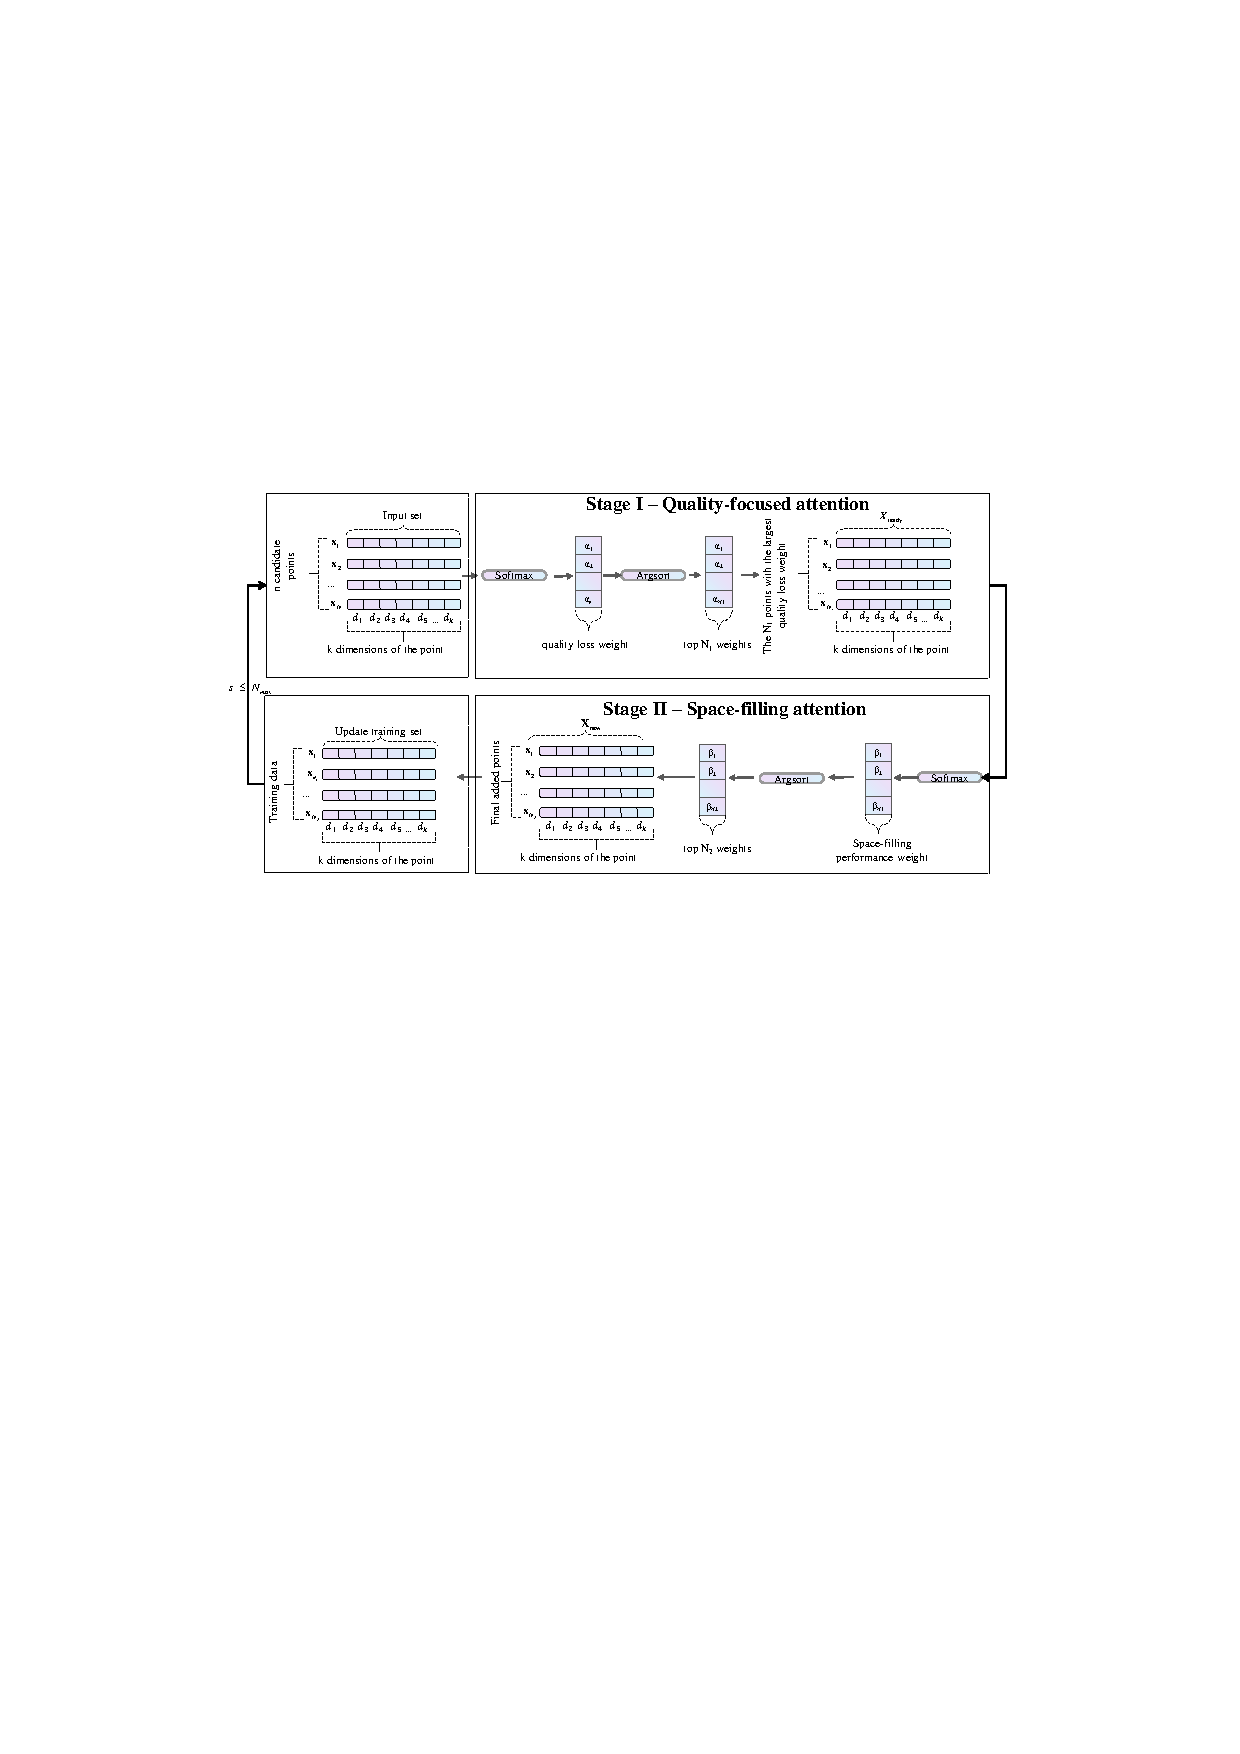
\includegraphics[width=0.9\linewidth]{FIG1.pdf}
	\caption{Attention-based active learning NSGP modeling procedure.}
	\label{fig:procedure}
\end{figure}

\subsection{Proposed robust optimization method}
The procedure of the proposed two-stage attention-based active learning method for NSGP modeling and parameter optimization is illustrated in Figure~2.
\begin{description}
	\item[Step 1:] Fit the initial NSGP model using the initial training samples.
	\item[Step 2:] Construct the quality loss function and the spatial distance
	function using the outputs of the initial model from Equations~(17)--(18).
	\item[Step 3:] Combine the two metrics from Step~2 to construct the two-stage
	attention-based acquisition function.
	\item[Step 4:] Apply the active learning process described in Algorithm~1 to
	select new design points.
	\item[Step 5:] Update the training dataset and the NSGP model, and obtain the
	predicted response mean and variance.
	\item[Step 6:] Formulate the quality loss function as the robust optimization
	objective using the predicted mean and variance from Step~5.
	\item[Step 7:] Employ the genetic algorithm (GA) to search for the global
	optimum within the feasible domain of the input variables, thereby
	determining the optimal parameter settings.
\end{description}
\begin{figure}[h!]
	\centering
	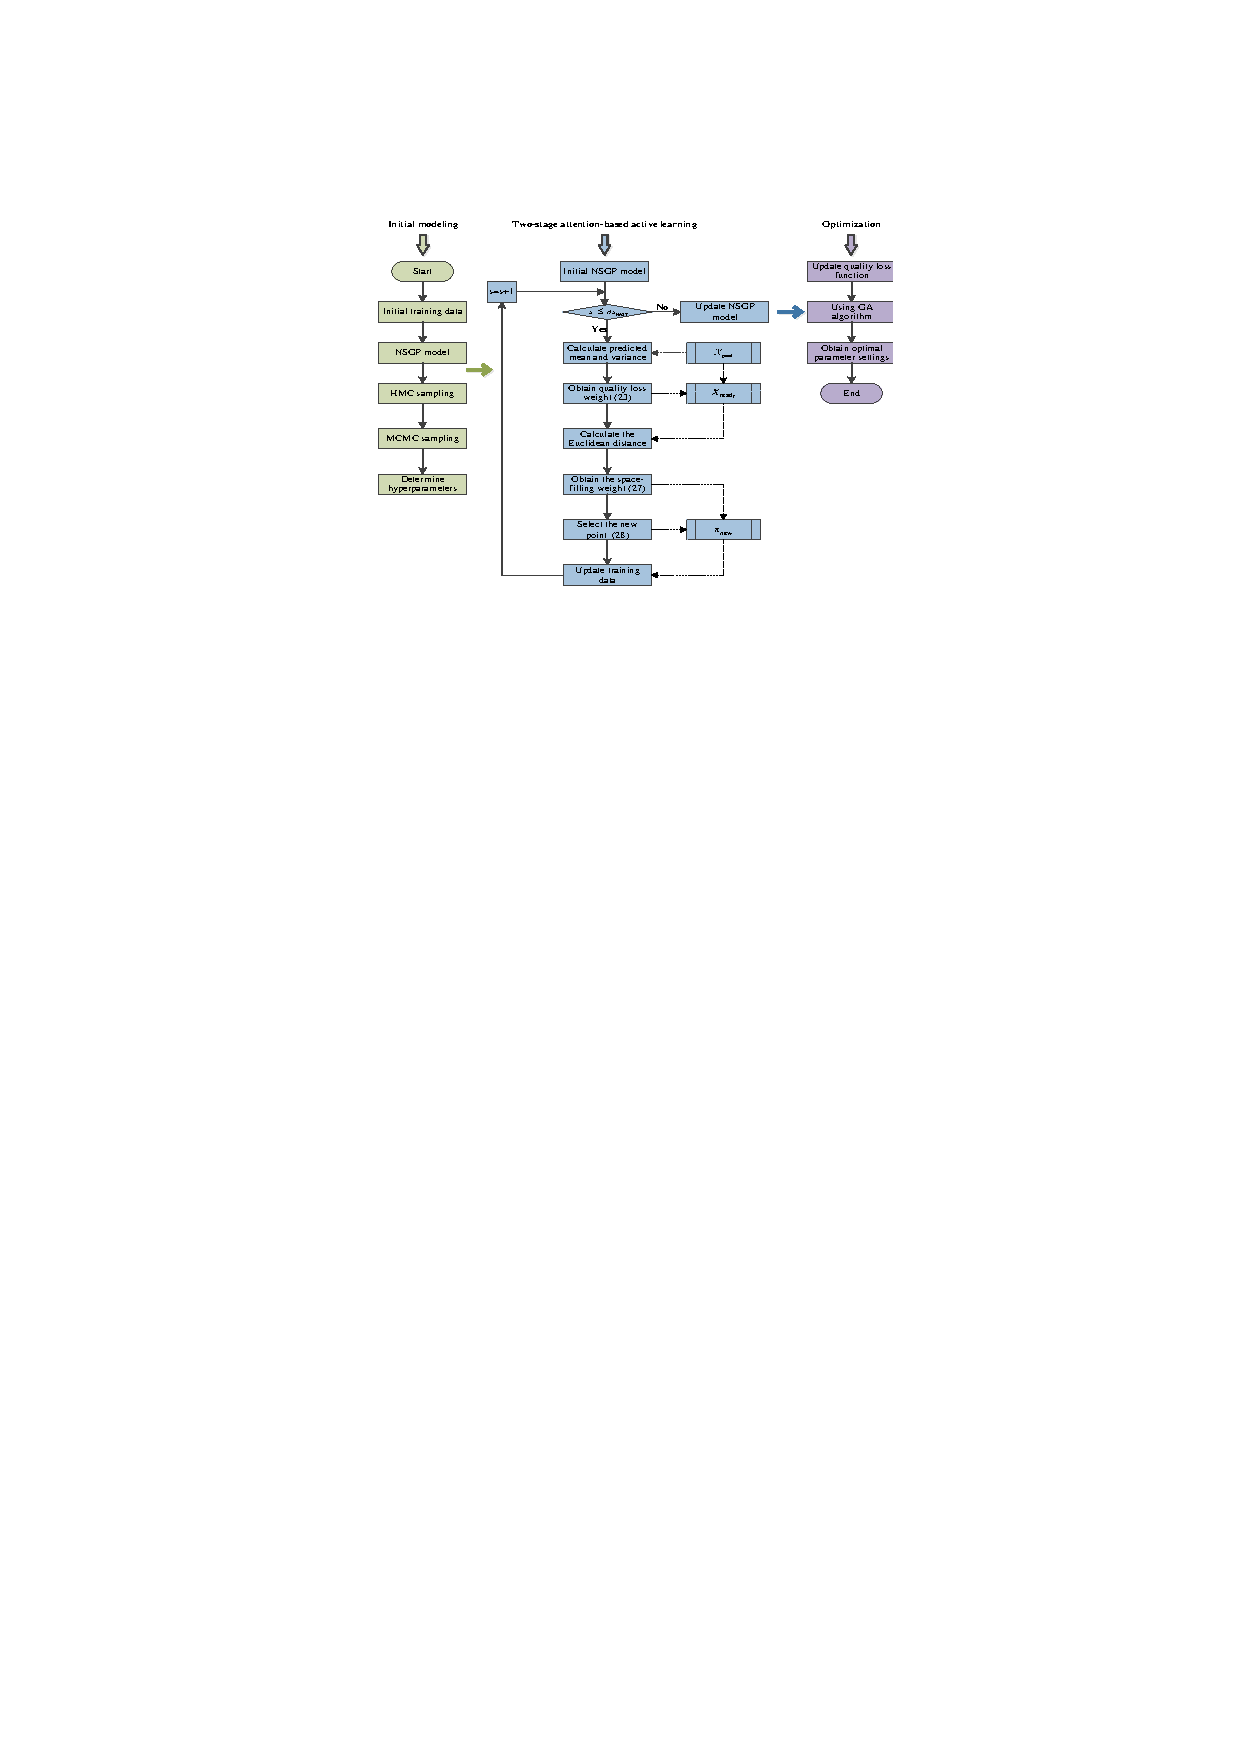
\includegraphics[width=0.8\linewidth]{FIG2.pdf}
	\caption{Flowchart of the proposed NSGP modeling and parameter optimization method.}
	\label{fig:fig2}
\end{figure}


\section{Case study}
\subsection{Two-dimensional numerical example}
This section validates the effectiveness of the proposed method using a two-dimensional test function. The function is a piecewise-defined response surface exhibiting pronounced nonstationarity in the two-dimensional input space. The mathematical expression of $f(x_{1}, x_{2})$ is given by:
\begin{equation}
	f({x_1},{x_2}) = \left\{ {\begin{array}{*{20}{l}}
			{(2 + 0.5{x_2})\sin ({x_1}) + x_2^2,}&{{\rm{if  }}{x_1} > 0},\\
			{x_1^2 + x_2^2 + \left( {8 - (x_1^2 + x_2^2)} \right)\left( {1 - {e^{ - x_1^2}}} \right),}&{{\rm{if  }}{x_1} \le 0},
	\end{array}} \right.
\end{equation}
where $(x_{1}, x_{2}) \in [-2, 2]^{2}$. For $x_{1} > 0$, the function exhibits periodic oscillations along the $x_{1}$ direction, whereas for $x_{1} \le 0$, it presents a circularly symmetric and smooth response. This behavior reflects significant nonstationarity and structural discontinuity. To further assess the local predictive performance of the model in the target region, a specific target value $f^{*}$ is defined for this test function. Around this target value, a region of interest ${\mathcal{R}}^{t}$ is defined as the set of input points satisfying: 
\begin{equation}
	{{\cal R}^t} = \left\{ {({x_1},{x_2}) \in {\cal X}\left| {\left| {f({x_1},{x_2}) - {f^*}} \right| < t} \right.} \right\},
\end{equation}
where $t > 0$ is a prescribed threshold. The set ${\mathcal{R}}^{t}$ can be regarded as the potential optimum subregion of the design space, within which the predictive accuracy is of critical importance for robust optimization. In this study, the target value is set to $f^{*} = 1.5$, which is deliberately chosen to avoid the extrema and thereby prevent misleading effects caused by extreme-value behavior. To quantify the discrepancy between predictions and the true values, the root mean square error (RMSE) is adopted as the performance metric, defined as:
\begin{equation}
	{\rm{RMSE}} = \sqrt {\frac{1}{n}\sum\limits_{i = 1}^n {{{\left( {\hat f(x_1^i,x_2^i) - f(x_1^i,x_2^i)} \right)}^2}} } ,
\end{equation}
where $\hat{f}(x_{1}^{i}, x_{2}^{i})$ denotes the model prediction, $f(x_{1}^{i}, x_{2}^{i})$ is the true value, and $n$ is the total number of test samples. In this experiment, $20$ initial design samples are first generated using Latin hypercube sampling (LHS) and employed to fit the initial NSGP model. Subsequently, $20$ additional samples are selected using the proposed two-stage attention-based active learning method, resulting in a final set of $40$ design points. The NSGP model is then updated using this final training data. For a direct comparison, several widely used experimental design methods are adopted as baseline approaches: the G\_optimality (G\_opt) method \citep{Omwando2024}, the D\_optimality (D\_opt) method \citep{Lichota2016}, the LHS method \citep{Guo2023}, and the centroidal Voronoi tessellations (CVT) method \citep{Vassiliades2018}. All methods use the same total number of samples. The spatial distributions of the $40$ design points obtained by the different methods in the two-dimensional design space are illustrated in Figure~3.
\begin{figure}[h]
	\centering
	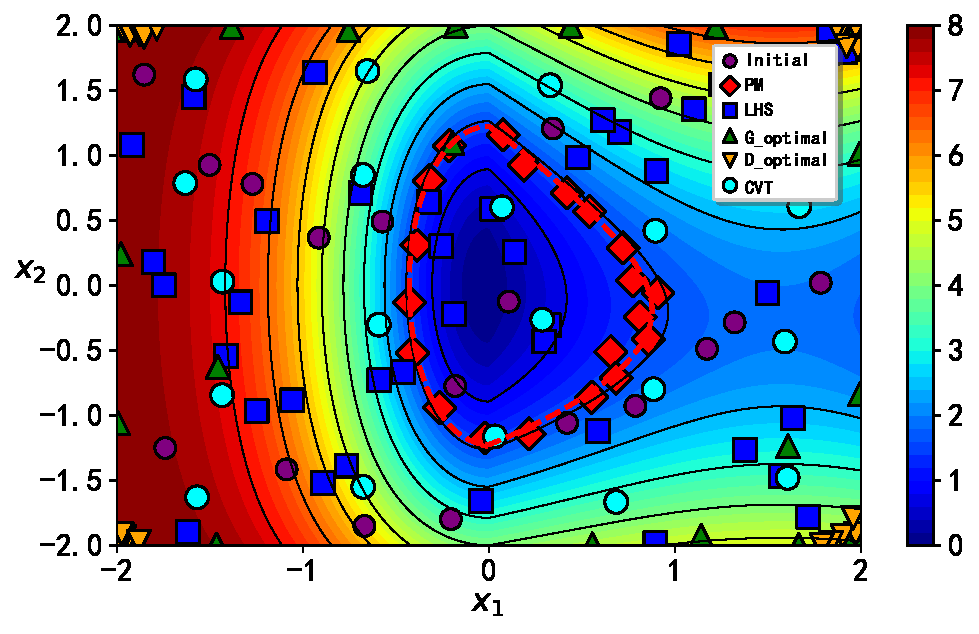
\includegraphics[width=0.7\linewidth]{FIG3.pdf}
	\caption{Spatial distribution of the 40 design points obtained by different methods.}
	\label{fig:design-points}
\end{figure}

In Figure 3, the purple circles represent the initial design points, whereas the red diamonds indicate the points selected using the proposed active learning method. The red dashed line depicts the contour corresponding to the target value of $1.5$. As shown, the design points selected by the proposed method (PM) are predominantly concentrated near the target-value contour. This distribution suggests that the algorithm tends to allocate experimental points to the potential optimum region. Furthermore, the design points close to the target contour exhibit a more uniform spatial distribution, with no apparent overlap or clustering. This characteristic demonstrates the favorable space-filling capability of the proposed active learning method. To further demonstrate the predictive accuracy advantage of the proposed approach, the RMSE values within the potential optimum region are evaluated. Comparisons are made across different total training sample sizes (40–100) and different numbers of newly added design points (20 and 10). For each method, the RMSE computation is repeated 30 times to ensure the reliability of the comparison. The results are summarized in Tables 1–2 and Figure 4. Specifically, Tables~1 and~2 report both the RMSE values and the corresponding improvement ratios of the proposed method over alternative approaches, based on 10 and 20 active learning design points, respectively. Other comparative results, including the maximum, minimum, first quartile (Q1), and third quartile (Q3), are provided in Appendix~A.

\begin{table}[h!]
	\centering
	\caption{RMSE results and PM improvement ratio with 10 active learning design points (PM improvement for PM is undefined and shown as ``—'').}
	\label{tab:rmse_pm_10pts}
	\resizebox{\linewidth}{!}{%
		\begin{tabular}{c ccccc c ccccc}
			\toprule
			\multirow{2}{*}{Number} & \multicolumn{5}{c}{RMSE (Mean)} & & \multicolumn{5}{c}{RMSE (Median)} \\
			\cmidrule(lr){2-6} \cmidrule(lr){8-12}
			& D\_opt & G\_opt & LHS & CVT & PM & & D\_opt & G\_opt & LHS & CVT & PM \\
			\midrule
			40  & 0.0919 & 0.0894 & 0.0780 & 0.0651 & 0.0562 & & 0.0854 & 0.0823 & 0.0675 & 0.0639 & 0.0503 \\
			50  & 0.0621 & 0.0650 & 0.0565 & 0.0560 & 0.0386 & & 0.0621 & 0.0663 & 0.0539 & 0.0586 & 0.0382 \\
			60  & 0.0514 & 0.0540 & 0.0451 & 0.0532 & 0.0369 & & 0.0487 & 0.0548 & 0.0448 & 0.0430 & 0.0362 \\
			70  & 0.0427 & 0.0442 & 0.0392 & 0.0365 & 0.0317 & & 0.0430 & 0.0419 & 0.0349 & 0.0357 & 0.0325 \\
			80  & 0.0369 & 0.0416 & 0.0330 & 0.0333 & 0.0246 & & 0.0365 & 0.0390 & 0.0320 & 0.0309 & 0.0241 \\
			90  & 0.0308 & 0.0323 & 0.0261 & 0.0296 & 0.0216 & & 0.0288 & 0.0317 & 0.0266 & 0.0264 & 0.0204 \\
			100 & 0.0225 & 0.0249 & 0.0238 & 0.0252 & 0.0181 & & 0.0228 & 0.0250 & 0.0228 & 0.0232 & 0.0192 \\
			\midrule
			\multirow{2}{*}{Number} & \multicolumn{5}{c}{PM Improvement (Mean, \%)} & & \multicolumn{5}{c}{PM Improvement (Median, \%)} \\
			\cmidrule(lr){2-6} \cmidrule(lr){8-12}
			& D\_opt & G\_opt & LHS & CVT & PM & & D\_opt & G\_opt & LHS & CVT & PM \\
			\midrule
			40  & 38.85\% & 37.14\% & 27.95\% & 13.67\% & — & & 41.10\% & 38.88\% & 25.48\% & 21.28\% & — \\
			50  & 37.84\% & 40.62\% & 31.68\% & 31.07\% & — & & 38.49\% & 42.38\% & 29.13\% & 34.81\% & — \\
			60  & 28.21\% & 31.67\% & 18.18\% & 30.64\% & — & & 25.67\% & 33.94\% & 19.20\% & 15.81\% & — \\
			70  & 25.76\% & 28.28\% & 19.13\% & 13.15\% & — & & 24.42\% & 22.43\% &  6.88\% &  8.96\% & — \\
			80  & 33.33\% & 40.87\% & 25.45\% & 26.13\% & — & & 33.97\% & 38.21\% & 24.69\% & 22.01\% & — \\
			90  & 29.87\% & 33.13\% & 17.24\% & 27.03\% & — & & 29.17\% & 35.65\% & 23.31\% & 22.73\% & — \\
			100 & 19.56\% & 27.31\% & 23.95\% & 28.17\% & — & & 15.79\% & 23.20\% & 15.79\% & 17.24\% & — \\
			\bottomrule
		\end{tabular}%
	}
\end{table}


% Requires: \usepackage{graphicx,booktabs}
\begin{table}[h!]
	\centering
	\caption{RMSE results and PM improvement ratio with 20 active learning design points (PM improvement for PM is undefined and shown as ``—'').}
	\label{tab:rmse_pm_20pts}
	\resizebox{\linewidth}{!}{%
		\begin{tabular}{c ccccc c ccccc}
			\toprule
			\multirow{2}{*}{Number} & \multicolumn{5}{c}{RMSE (Mean)} & & \multicolumn{5}{c}{RMSE (Median)} \\
			\cmidrule(lr){2-6} \cmidrule(lr){8-12}
			& D\_opt & G\_opt & LHS & CVT & PM & & D\_opt & G\_opt & LHS & CVT & PM \\
			\midrule
			40  & 0.1517 & 0.0954 & 0.0730 & 0.0817 & 0.0540 & & 0.1385 & 0.0890 & 0.0644 & 0.0802 & 0.0310 \\
			50  & 0.0990 & 0.0530 & 0.0538 & 0.0719 & 0.0324 & & 0.0954 & 0.0530 & 0.0510 & 0.0730 & 0.0249 \\
			60  & 0.0499 & 0.0481 & 0.0396 & 0.0565 & 0.0216 & & 0.0481 & 0.0458 & 0.0390 & 0.0562 & 0.0207 \\
			70  & 0.0453 & 0.0410 & 0.0359 & 0.0511 & 0.0235 & & 0.0466 & 0.0422 & 0.0356 & 0.0503 & 0.0222 \\
			80  & 0.0345 & 0.0400 & 0.0359 & 0.0419 & 0.0223 & & 0.0367 & 0.0378 & 0.0347 & 0.0431 & 0.0205 \\
			90  & 0.0319 & 0.0298 & 0.0263 & 0.0391 & 0.0187 & & 0.0298 & 0.0310 & 0.0263 & 0.0377 & 0.0180 \\
			100 & 0.0281 & 0.0321 & 0.0227 & 0.0354 & 0.0173 & & 0.0281 & 0.0328 & 0.0230 & 0.0352 & 0.0164 \\
			\midrule
			\multirow{2}{*}{Number} & \multicolumn{5}{c}{PM Improvement (Mean, \%)} & & \multicolumn{5}{c}{PM Improvement (Median, \%)} \\
			\cmidrule(lr){2-6} \cmidrule(lr){8-12}
			& D\_opt & G\_opt & LHS & CVT & PM & & D\_opt & G\_opt & LHS & CVT & PM \\
			\midrule
			40  & 64.40\% & 43.40\% & 26.03\% & 33.90\% & — & & 77.62\% & 65.17\% & 51.86\% & 61.35\% & — \\
			50  & 67.27\% & 38.87\% & 39.78\% & 54.94\% & — & & 73.90\% & 53.02\% & 51.18\% & 65.89\% & — \\
			60  & 56.71\% & 55.09\% & 45.45\% & 61.77\% & — & & 56.96\% & 54.80\% & 46.92\% & 63.17\% & — \\
			70  & 48.12\% & 42.68\% & 34.54\% & 54.01\% & — & & 52.36\% & 47.39\% & 37.64\% & 55.86\% & — \\
			80  & 35.36\% & 44.25\% & 37.88\% & 46.78\% & — & & 44.14\% & 45.77\% & 40.92\% & 52.44\% & — \\
			90  & 41.38\% & 37.25\% & 28.90\% & 52.17\% & — & & 39.60\% & 41.94\% & 31.56\% & 52.25\% & — \\
			100 & 38.43\% & 46.11\% & 23.79\% & 51.13\% & — & & 41.64\% & 50.00\% & 28.70\% & 53.41\% & — \\
			\bottomrule
		\end{tabular}%
	}
\end{table}

\begin{figure}[h!]
	\centering
	% --- Top row: Potential optimum subregion ---
	\subfigure[10 active learning points.]{%
		\resizebox*{5cm}{!}{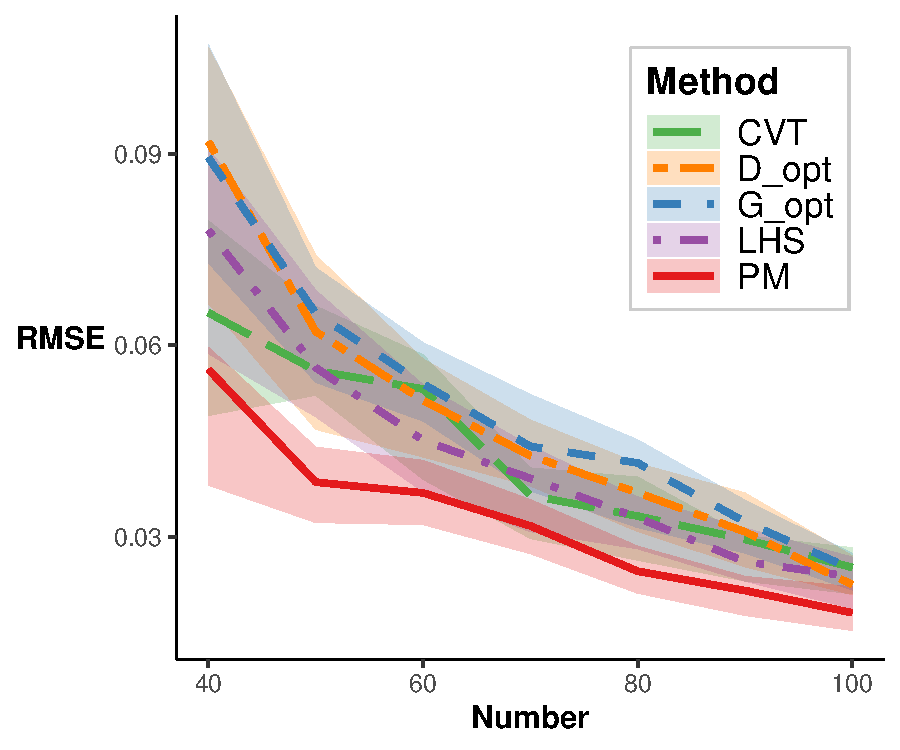
\includegraphics{FIG4a.pdf}}}\hspace{15pt}
	\subfigure[20 active learning points.]{%
		\resizebox*{5cm}{!}{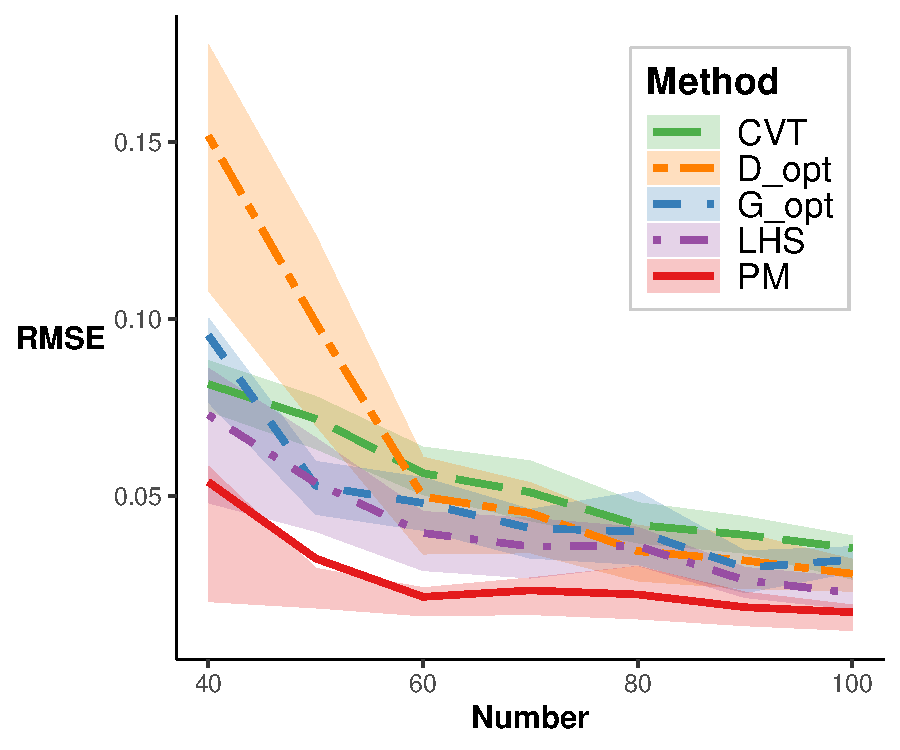
\includegraphics{FIG4b.pdf}}}
	
	% --- Bottom row: Overall response surface ---
	\subfigure[10 active learning points.]{%
		\resizebox*{5cm}{!}{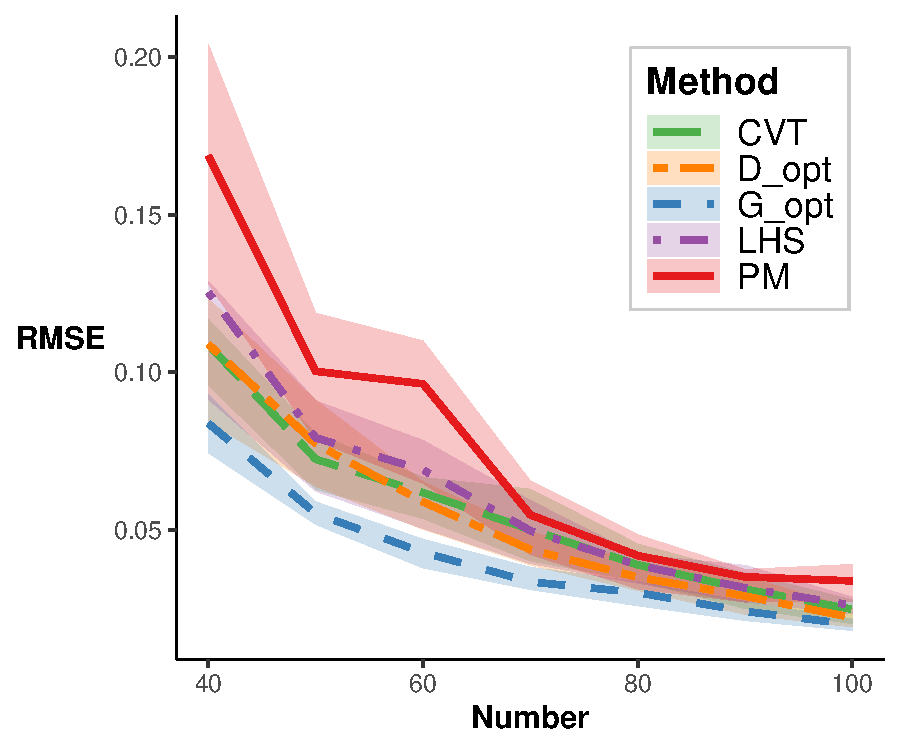
\includegraphics{FIG5a.pdf}}}\hspace{15pt}
	\subfigure[20 active learning points.]{%
		\resizebox*{5cm}{!}{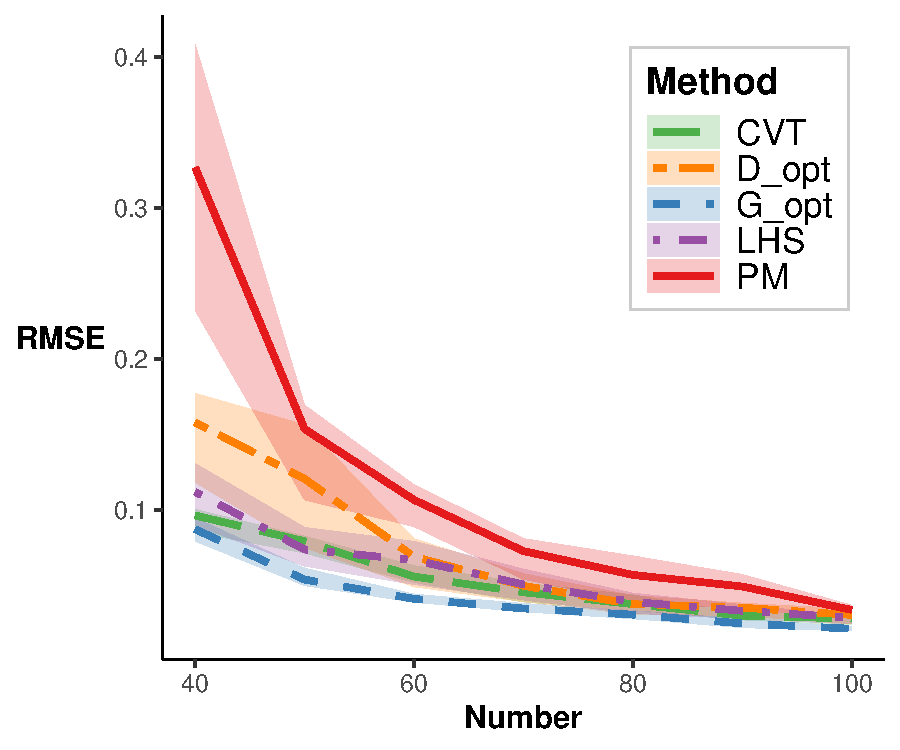
\includegraphics{FIG5b.pdf}}}
	
	\caption{Comparison of RMSE with different numbers of active learning design points: 
		(a)–(b) potential optimum subregion; 
		(c)–(d) overall response surface.}
	\label{fig:rmse_combined}
\end{figure}

Based on the results in Table 1 and Figures 4(a-b), when ten active learning design points are used, the PM method achieves the lowest mean RMSE in the potential optimum region across all training sample sizes. When the total number of experimental samples is 40, the PM method attains a mean RMSE of 0.0562. This is approximately 13.67\% lower than the CVT method (0.0651) and about 38.85\% lower than the D\_opt method (0.0919). The advantage remains as the sample size increases. When the total number of samples reaches 100, the mean RMSE of the PM method further decreases to 0.0181, representing a 19.56\% reduction compared with the D\_opt method (0.0225) and a 28.17\% reduction compared with the CVT method (0.0252). Among all comparisons, the largest improvement is observed when the training sample size is 80, compared with the D\_opt method, with a gain of 40.87\%. The smallest improvement occurs when the training sample size is 70, compared with the CVT method, with a gain of 13.15\%.
The median RMSE reflects the typical performance of the model. The PM method also performs strongly under this metric, indicating the high robustness of its results. With ten active learning design points and a total of 40 experimental samples, the median RMSE of the PM method is $0.0503$. This is approximately $21.28\%$ lower than that of the CVT method ($0.0639$) and about $41.10\%$ lower than that of the D\_opt method ($0.0854$). When the total number of experimental samples reaches $100$, the PM method achieves a median RMSE of $0.0192$. This represents a $15.79\%$ reduction compared with both the D\_opt and LHS methods ($0.0228$ each), and a $23.20\%$ reduction compared with the G\_opt method ($0.0250$). The largest improvement is observed when the training sample size is $50$ compared with the G\_opt method, with a gain of $42.38\%$. The smallest improvement occurs when the training sample size is $70$ compared with the LHS method, with a gain of $6.88\%$.
From Table 2 and Figures 4(a-b), when 20 active learning samples are added, the PM method outperforms the alternatives in terms of RMSE across all cases. The advantage is particularly evident in the early learning stage when the total sample size is small. With a total of 40 experimental samples, the PM method achieves a mean RMSE of $0.0540$, which is approximately $26.03\%$ lower than LHS ($0.0730$) and $64.40\%$ lower than D\_opt ($0.1517$). When the total sample size increases to $100$, the mean RMSE of the PM method decreases to $0.0173$, which remains the lowest in Table 2. For this sample size, the value is $23.79\%$ lower than LHS ($0.0227$) and $51.13\%$ lower than CVT ($0.0354$). Across all sample sizes, the largest improvement is observed when the sample size is $50$ compared with D\_opt, with a gain of $67.27\%$. The smallest improvement is observed when the sample size is $100$ compared with LHS, with a gain of $23.79\%$.

When the number of active learning samples is 20, the PM method also demonstrates a clear advantage in terms of the median RMSE. With a total sample size of 40, the median RMSE is $0.0310$. This is $51.86\%$ lower than the second-best LHS method ($0.0644$) and $77.62\%$ lower than the D\_opt method ($0.1385$). When the total sample size increases to 100, the median RMSE of the PM method is $0.0164$, the lowest among all methods. At this size, it is $28.70\%$ lower than the LHS method ($0.0230$) and $53.41\%$ lower than the CVT method ($0.0352$). The largest improvement occurs with 40 training samples compared with the D\_opt method, reaching $77.62\%$. The smallest improvement is seen with 100 training samples compared with the LHS method, at $28.70\%$.

The comparative results in the tables and figures indicate that the proposed PM method achieves a clear advantage in predictive accuracy within the potential optimum region. This advantage mainly arises from its two-stage attention mechanism. In the first stage, design points are selected to substantially improve predictive accuracy in the potential optimum region. In the second stage, a spatial-distance criterion is applied to suppress local clustering, thereby enhancing space-filling in that region. By contrast, the G\_opt method improves prediction by minimizing the maximum prediction variance across the design space. The D\_opt method seeks to optimize overall parameter estimation accuracy by maximizing the determinant of the information matrix. The LHS method focuses on evenly distributing samples in each input dimension to achieve full coverage of the design space. The CVT method ensures uniform sampling density by moving sample points toward the centroids of their Voronoi cells. Consequently, under various conditions, these methods yield lower predictive accuracy in the potential optimum region than the PM method.

It is noteworthy that, in terms of the overall response surface prediction accuracy (Figures 4(c-d)), the RMSE of the PM method is slightly higher than that of the alternative approaches. This difference occurs because the PM method allocates new design points to the most promising potential optimum region for robust optimization. Such allocation inevitably sacrifices part of the global prediction accuracy. However, the results in Figure 4 show that the decrease in global accuracy is much smaller than the improvement achieved in the potential optimum region. Robust optimization places greater emphasis on prediction accuracy within the optimum region. Therefore, this local improvement is more important for obtaining high-quality and stable solutions. Although the PM method incurs a small loss in global accuracy, it significantly enhances the prediction accuracy in the potential optimum region. This improvement enhances the quality, stability, and validity of solutions in robust parameter design.

\subsection{Five-dimensional numerical example}
In practical applications, multiple variables often exhibit complex and nonlinear interactions. To evaluate the applicability and advantages of the proposed method in high-dimensional settings, a five-dimensional piecewise-defined numerical test function is considered:

\begin{equation}
	y = \left\{ {\begin{array}{*{20}{l}}
			{2\left( {\sin (\pi {x_1}) + \cos (2\pi {x_2}) + x_3^2 + {e^{ - {x_4}}} + {x_5} + {x_3} - 1} \right)},&{{\rm{if }}{x_1} + {x_2} > 1,}&{}\\
			{2\left( {\sin (\pi {x_1}) + \cos (2\pi {x_2}) + x_3^2 + {e^{ - {x_4}}} + {x_5} - 1} \right)},&{{\rm{if }}{x_1} + {x_2} \le 1},&{}
	\end{array}} \right.
\end{equation}
where $x_g \in [0, 1],\ g = 1, 2, \ldots, 5$.  The function exhibits a structural change between the two subregions $x_{1} + x_{2} > 1$ and $x_{1} + x_{2} \le 1$, leading to distinct output behaviors and representing typical input-dependent nonstationarity. In this example, the target value is set to $5.5$, and the optimum region is defined as $5 \le y \le 6$. The RMSE is employed to evaluate predictive accuracy within this region. The experimental procedure is as follows: first, $80$ initial experimental samples are selected using the LHS method to fit the NSGP model; second, $20$ additional samples are generated using the proposed two-stage active learning method with the attention mechanism, yielding a total of $100$ samples; finally, this process is repeated $30$ times, and the RMSE results in the optimum region are compared with those of multiple alternative methods. The results are reported in Table 3 and Figure 5.

\begin{table}[h]
	\centering
	\caption{RMSE results within the optimum region ($5 \le y \le 6$)}
	\label{tab:rmse_optimum_region}
		\begin{tabular}{lccccccc}
			\toprule
			Method & Mean & Median & Min & Max & Q1 & Q3 \\
			\midrule
			D\_opt & 0.4075 & 0.4107 & 0.2340 & 0.5197 & 0.3665 & 0.4539 \\
			G\_opt & 0.4146 & 0.4025 & 0.2901 & 0.5934 & 0.3497 & 0.4806 \\
			CVT    & 0.4372 & 0.4360 & 0.3162 & 0.5928 & 0.3870 & 0.4762 \\
			LHS    & 0.4372 & 0.4447 & 0.3256 & 0.7144 & 0.3804 & 0.4860 \\
			PM     & 0.3711 & 0.3793 & 0.2239 & 0.4921 & 0.3102 & 0.4189 \\
			\bottomrule
		\end{tabular}%
\end{table}

\begin{figure}[h]
	\centering
	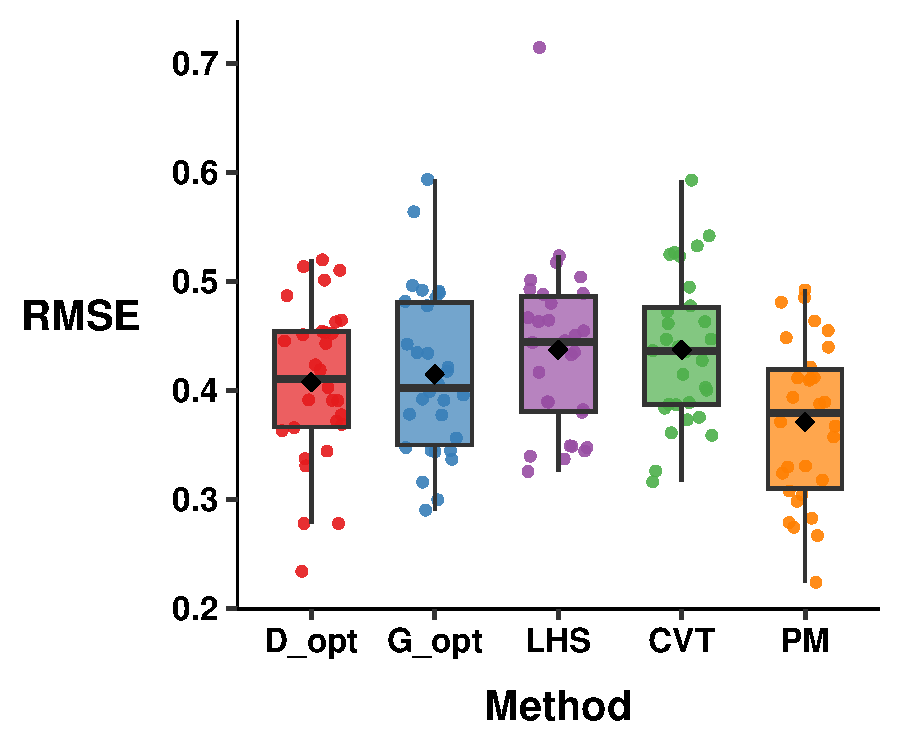
\includegraphics[width=0.48\linewidth]{FIG6.pdf}
	\caption{Comparison of RMSE results within the optimum region ($5 \le y \le 6$).}
	\label{fig:rmse_optimum_region}
\end{figure}

As shown in Table 3, the PM method attains a mean RMSE of $0.3711$, outperforming all alternative approaches. The D\_opt method ranks second with $0.4075$, whereas the G\_opt method records the highest mean RMSE at $0.4146$. Relative to D\_opt and G\_opt, the PM method achieves reductions of approximately $8.93\%$ and $10.49\%$, respectively. Compared with LHS and CVT, both with a mean RMSE of $0.4372$, the reduction reaches $15.12\%$. For the median RMSE, the PM method again delivers the best performance ($0.3793$), representing reductions of $5.76\%$ compared with G\_opt ($0.4025$), $7.65\%$ compared with D\_opt ($0.4107$), $13.00\%$ compared with LHS ($0.4360$), and $14.71\%$ compared with CVT ($0.4447$). The consistent advantage in both mean and median RMSE underscores the stability and overall superiority of the PM method. This performance is driven by its two-stage active learning framework with an attention mechanism. In the first stage, a quality loss-based acquisition function is applied to refine the response surface representation within the optimum region. In the second stage, the design maximizes the minimum spatial distance, reducing local clustering and improving space-filling in the region. This design substantially increases the efficiency of experimental resource utilization in robust optimization and yields a more effective nonstationary response surface model.

\subsection{Lithium battery state-of-charge prediction}
This section adopts the lithium battery state-of-charge (SoC) prediction case study presented by \cite{Mustafa2024} to evaluate the performance of the proposed method. During different stages of battery discharge, the SoC exhibits markedly different response rates to current and voltage, demonstrating typical nonstationary behavior. Using an 18650-type lithium-ion battery as the study object, the case involves one output variable—SoC (\%). SoC is defined as the percentage of the current charge relative to the total capacity of the battery, ranging from $y \in [0,100]$, and serves as a key indicator for evaluating the remaining capacity of the battery. This case study inputs include three variables: temperature $x_1$ (°C), current $x_2$ (A), and voltage $x_3$ (V). In this experiment, the SoC target value is set to $30$, and the optimum region is defined as $25 \le y \le 35$. First, 180 initial training points are generated using the LHS method. The additional 30 points are then selected with the proposed two-stage active learning algorithm, resulting in a total of 210 experimental samples. The entire process is repeated 20 times to ensure robustness of the results. Table 4 and Figure 6 show the RMSE results for the optimum region from different methods.

\begin{table}[htbp]
	\centering
	\caption{RMSE results from 20 runs.}
	\label{tab:rmse_20runs}
		\begin{tabular}{lcccccc}
			\toprule
			Method & Mean & Median & Max & Min & Q1 & Q3 \\
			\midrule
			G\_opt & 7.9793 & 6.8957 & 18.3144 & 5.5627 & 6.0980 & 8.3195 \\
			D\_opt & 7.8077 & 7.0209 & 15.5626 & 5.9420 & 6.7881 & 7.6917 \\
			CVT    & 10.7557 & 9.2375 & 26.6414 & 6.9491 & 7.2289 & 12.0859 \\
			LHS    & 9.2725 & 7.6885 & 16.9593 & 6.4247 & 7.0761 & 10.5335 \\
			PM     & 6.9880 & 6.7256 & 10.9925 & 4.8605 & 6.1098 & 7.3933 \\
			\bottomrule
		\end{tabular}
\end{table}

\begin{figure}[htbp]
	\centering
	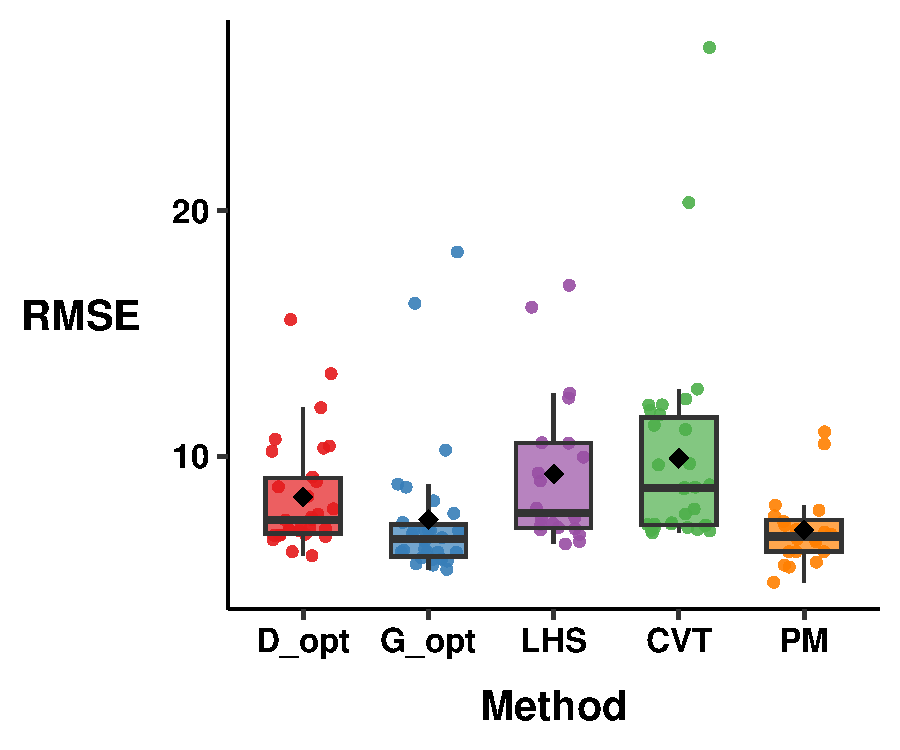
\includegraphics[width=0.48\linewidth]{FIG7.pdf}
	\caption{Comparison of battery SoC prediction results.}
	\label{fig:battery_soc_comparison}
\end{figure}

Table 4 and Figure 6 show that the PM method achieves the highest predictive accuracy within the optimum region. Its mean RMSE is $6.9880$, which is markedly lower than all baseline methods. The CVT method records the highest mean RMSE ($10.7557$), with a gap of $35.03\%$ compared with the PM method, while the second-best D\_opt method ($7.8077$) still lags by $10.50\%$. The median RMSE results align with the mean trends: the PM method again attains the lowest value ($6.7256$), $27.19\%$ lower than that of CVT ($9.2375$), indicating its ability to maintain high predictive accuracy in most trials. Beyond central tendency, the PM method also excels in controlling extreme values. Its maximum RMSE is only $10.9925$, which is $58.74\%$ lower than the CVT method’s $26.6414$, demonstrating effective suppression of extreme errors. ts minimum RMSE of $4.8605$ outperforms all other methods, being $30.05\%$ lower than the minimum RMSE of CVT ($6.9491$), suggesting a greater tendency to converge to high-accuracy solutions during the search process. In terms of stability, the PM method achieves an interquartile range (IQR) of $1.2835$, only $26.43\%$ of that of CVT ($4.8570$), representing a $73.57\%$ reduction. This further confirms that the PM method attains high robustness without compromising accuracy. As illustrated in Figure 6, the RMSE distribution of the PM method is more concentrated, with fewer outliers, validating its combined advantage in predictive accuracy and robustness within the optimum region.


\subsection{Robust parameter design for a micro-rocket}

This section adopts the micro-rocket design case study introduced by \cite{Box2011} to validate the effectiveness and advantages of the proposed method in product quality design. The rocket model consists of a nose cone, fuselage, launch damper lock with parachute, inner tube, and stabilizing fins, as shown in Figure 7. The output response is the maximum flight height (MH)  $y$ (m), which serves as a key indicator for evaluating the overall performance of the rocket. Analyzing the maximum altitude provides an integrated measure of thrust, aerodynamic drag, and structural design performance. In this case, the target value is set to 400 m, representing a typical nominal-the-best quality characteristic. The simulated flight trajectory and the relationship between maximum flight altitude and nose cone diameter are presented in Figures 8(a) and 8(b), respectively.

\begin{figure}[h!]
	\centering
	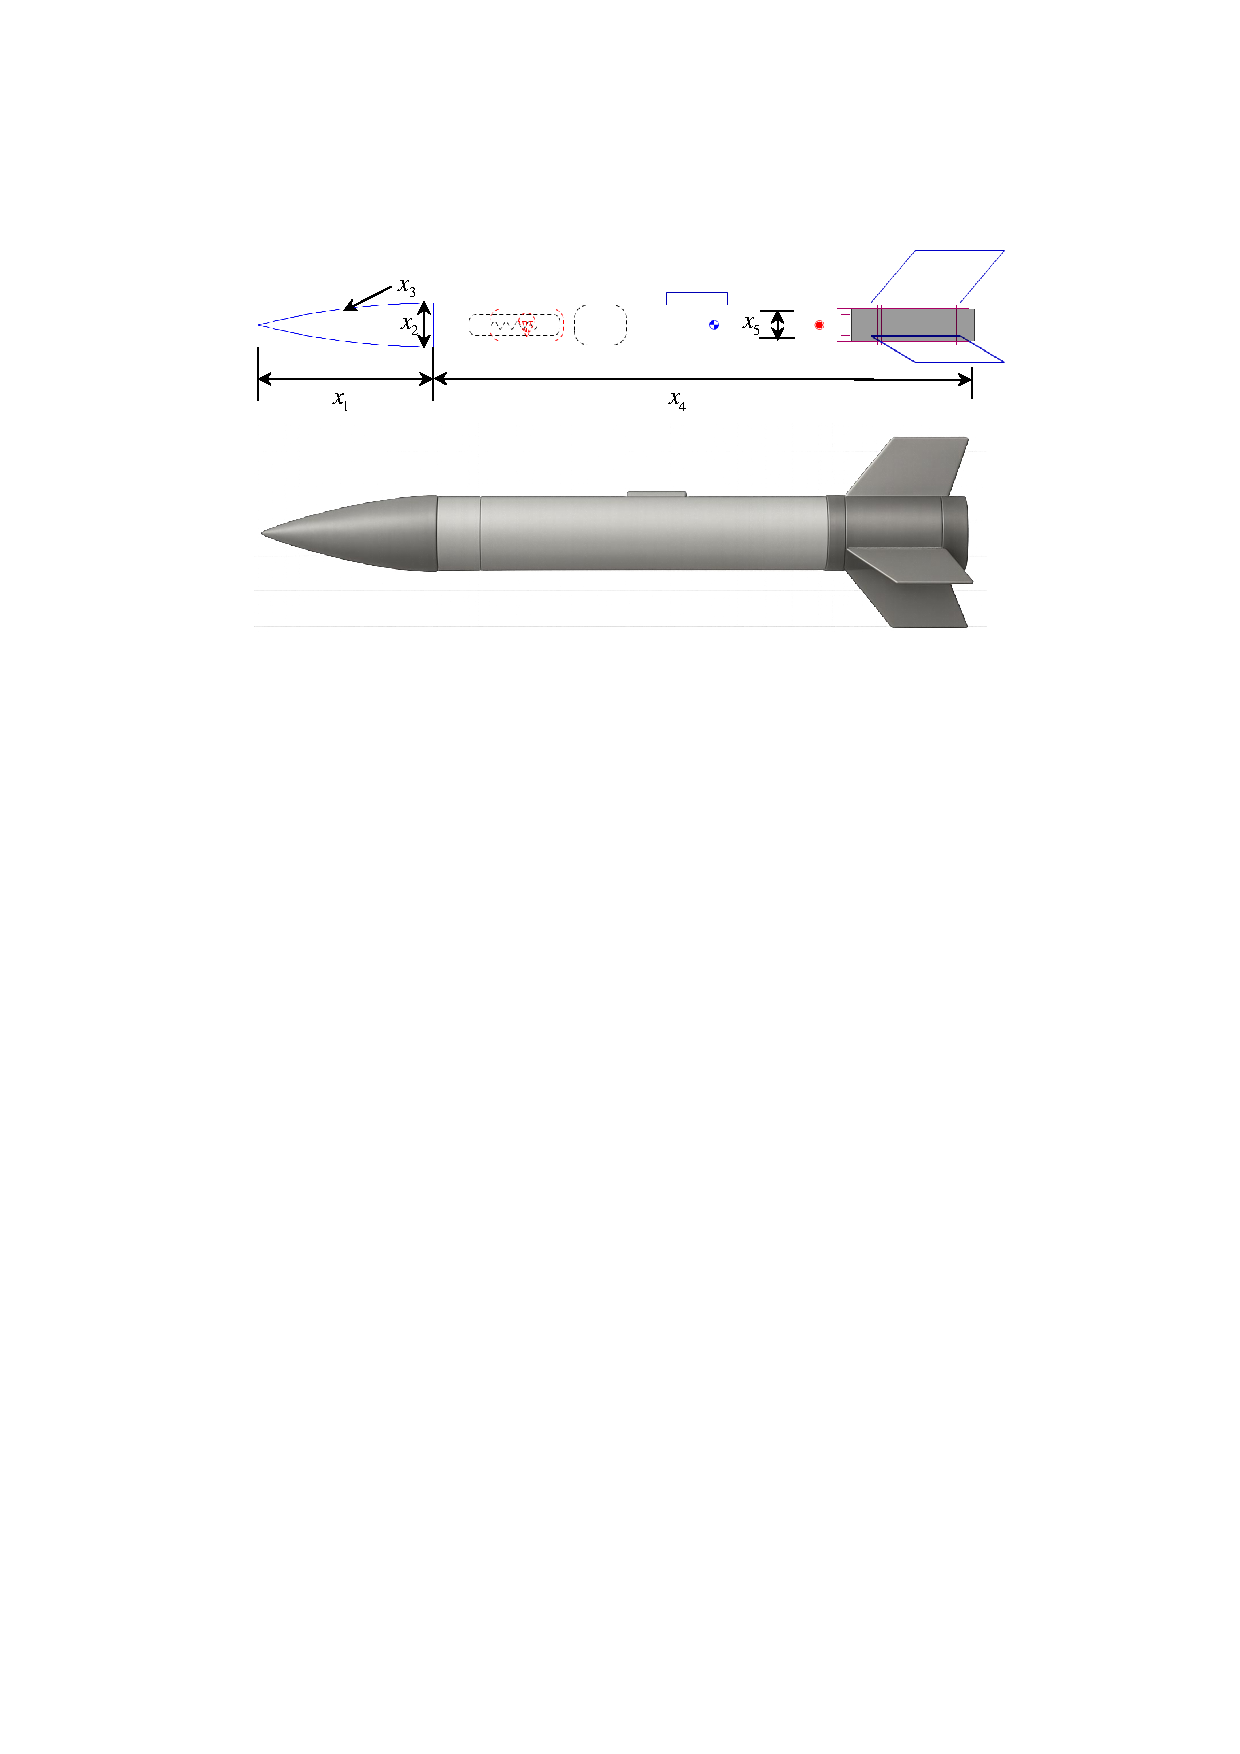
\includegraphics[width=0.7\linewidth]{FIG8.pdf}% 
	\caption{Rocket model diagram.}
	\label{fig:rocket_model}
\end{figure}

\begin{figure}[h!]
	\centering
	\subfigure[Schematic of rocket flight trajectory.]{%
		\resizebox*{0.4\linewidth}{!}{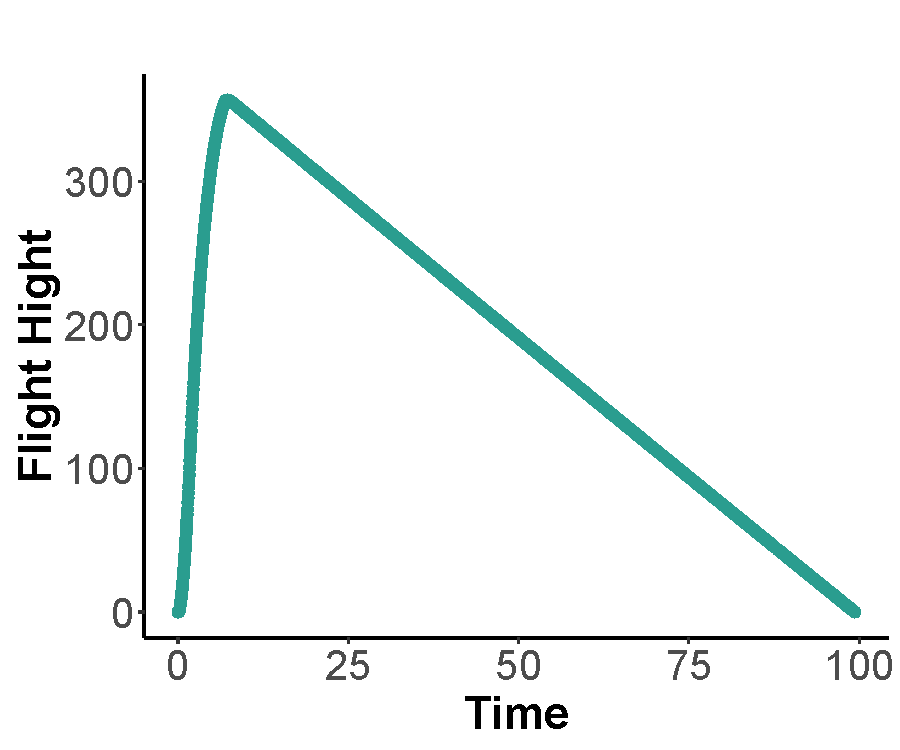
\includegraphics{FIG9a.pdf}}%
	}\hspace{5pt}
	\subfigure[MH and nose cone diameter.]{%
		\resizebox*{0.4\linewidth}{!}{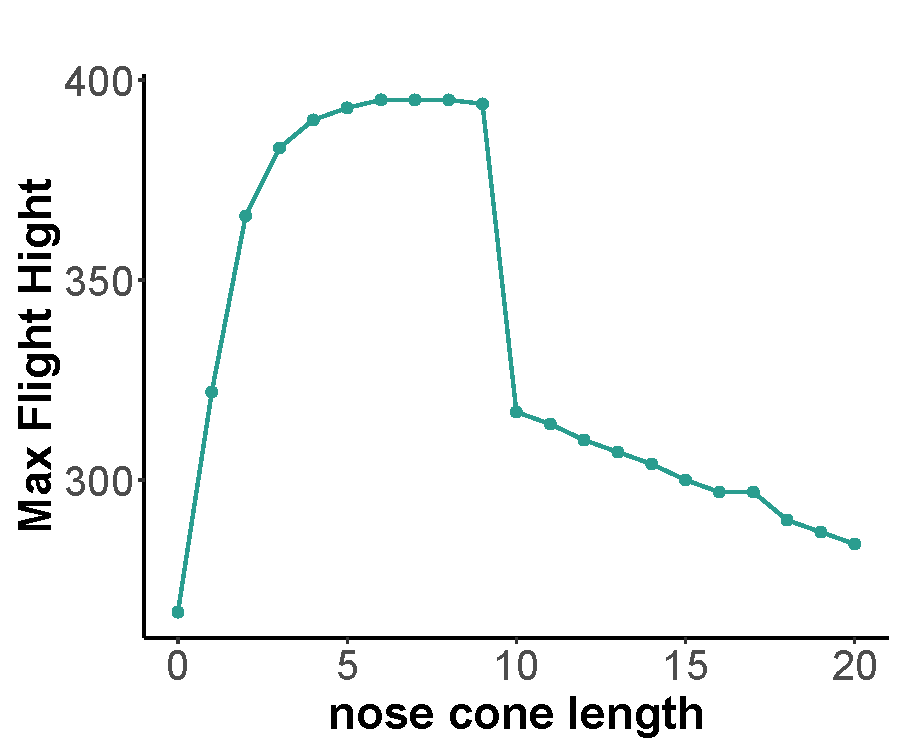
\includegraphics{FIG9b.pdf}}%
	}
	\caption{Simulated flight trajectory and the relationship between MH and nose cone diameter.}
	\label{fig:rocket_traj_pair}
\end{figure}

The case study involves five continuous input parameters: nose cone length $x_{1}$ (cm), base diameter of the nose cone $x_{2}$ (cm), nose cone wall thickness $x_{3}$ (cm), fuselage length $x_{4}$ (cm), and inner diameter of the fuselage $x_{5}$ (cm). Their respective ranges are $x_{1} \in [0,20]$, $x_{2} \in [2,5]$, $x_{3} \in [0,1]$, $x_{4} \in [30,50]$, and $x_{5} \in [1,2]$. In addition, there is one binary discrete variable—the nose cone shape $x_{6}$—where $x_{6} = 1$ denotes an ogive with a cut tip, and $x_{6} = 0$ denotes an ogive with a truncated tip. According to the design specifications, for longer nose cones ($x_{1} > 10$ cm), the cut-tip ogive is preferred to reduce shock wave drag during supersonic flight, thereby improving aerodynamic performance and enhancing stability. For shorter nose cones ($x_{1} < 10$ cm), the truncated-tip ogive is selected to increase lift and improve stability in subsonic flight. This shape transition at $x_{1} = 10$ cm introduces a distinct structural change, causing a step-like behavior in the output response at this location and resulting in a pronounced nonstationary characteristic. 

The objective of robust parameter design in this case study is to identify an optimal combination of design parameters that enables the rocket to achieve a maximum flight altitude of $400$ m or as close as possible to this target. To this end, the subsequent experiments employ the proposed method to improve the predictive accuracy within the potential optimum region, thereby constructing a more efficient and stable nonstationary response surface model. The experimental procedure is as follows: first, $30$ initial training points are selected using the LHS method, and an initial NSGP-based nonstationary response surface model is fitted. Next, $20$ additional design points are generated using the proposed two-stage active learning algorithm, bringing the total number of training samples to $50$, as shown in Table 5.

\begin{table}[h!]
	\centering
	\caption{Experimental results of the PM method.}
	\label{tab:pm_runs}
	\resizebox{\linewidth}{!}{%
		\begin{tabular}{c cccccc c c cccccc cc}
			\toprule
			\multicolumn{8}{c}{Runs 1--25} & & \multicolumn{8}{c}{Runs 26--50} \\
			\cmidrule(lr){1-8} \cmidrule(lr){10-17}
			Run & $x_1$ & $x_2$ & $x_3$ & $x_4$ & $x_5$ & $x_6$ & $y$ & & Run & $x_1$ & $x_2$ & $x_3$ & $x_4$ & $x_5$ & $x_6$ & $y$ \\
			\midrule
			1 & 15.5 & 3.13 & 0.96 & 48.8 & 1.89 & 1 & 26.7  & & 26 &  9.9 & 2.20 & 0.02 & 38.4 & 1.62 & 0 & 262    \\
			2 & 12.9 & 2.81 & 0.07 & 41.3 & 1.96 & 1 & 130    & & 27 & 14.2 & 2.91 & 0.28 & 38.6 & 1.86 & 1 &  87.5  \\
			3 &  1.3 & 2.06 & 0.63 & 37.4 & 1.31 & 0 & 227    & & 28 & 16.6 & 2.71 & 0.90 & 40.9 & 1.38 & 1 &  50.5  \\
			4 &  0.5 & 3.97 & 0.10 & 45.6 & 1.23 & 0 &  7.59  & & 29 & 17.2 & 3.32 & 0.44 & 30.8 & 1.14 & 1 &  33.6  \\
			5 & 10.7 & 4.17 & 0.13 & 33.9 & 1.86 & 1 &  1.1   & & 30 &  5.2 & 4.50 & 1.00 & 32.0 & 1.54 & 0 &   9.25 \\
			6 & 18.7 & 4.81 & 0.86 & 36.7 & 1.18 & 1 &  0.39  & & 31 &  0.7 & 2.08 & 0.25 & 30.7 & 1.92 & 0 & 373.89 \\
			7 & 17.9 & 3.85 & 0.65 & 47.0 & 1.49 & 1 &  4.59  & & 32 &  4.9 & 2.03 & 0.16 & 34.8 & 1.88 & 0 & 358.91 \\
			8 &  2.6 & 2.39 & 0.83 & 45.5 & 1.53 & 0 & 146    & & 33 &  5.8 & 2.12 & 0.02 & 30.2 & 1.97 & 0 & 369.85 \\
			9 &  2.0 & 4.69 & 0.67 & 32.9 & 1.15 & 0 &  5.65  & & 34 &  8.7 & 2.02 & 0.19 & 33.4 & 1.89 & 0 & 362.51 \\
			10 & 11.1 & 4.97 & 0.14 & 44.2 & 1.92 & 1 &  0.64  & & 35 & 10.5 & 2.03 & 0.35 & 31.3 & 1.86 & 1 & 358.85 \\
			11 & 18.0 & 3.99 & 0.82 & 40.6 & 1.98 & 1 &  7.19  & & 36 &  0.4 & 2.04 & 0.77 & 34.9 & 1.95 & 0 & 365.41 \\
			12 &  2.0 & 2.96 & 0.24 & 42.6 & 1.33 & 0 &  6.25  & & 37 &  4.0 & 2.05 & 0.17 & 32.8 & 1.85 & 0 & 358.41 \\
			13 & 17.3 & 4.63 & 0.91 & 43.3 & 1.00 & 1 &  0.27  & & 38 &  2.1 & 2.08 & 0.45 & 35.6 & 1.99 & 0 & 359.29 \\
			14 & 11.2 & 3.71 & 0.32 & 33.5 & 1.72 & 1 & 29     & & 39 &  6.8 & 2.12 & 0.07 & 33.5 & 1.99 & 0 & 358.02 \\
			15 &  8.1 & 3.75 & 0.50 & 35.8 & 1.69 & 0 & 24.6   & & 40 & 10.3 & 2.03 & 0.08 & 36.1 & 1.89 & 1 & 348.89 \\
			16 & 15.6 & 2.50 & 0.23 & 47.4 & 1.26 & 1 & 77.6   & & 41 &  2.0 & 2.04 & 0.89 & 33.6 & 1.84 & 0 & 349.3  \\
			17 &  7.5 & 3.15 & 0.44 & 31.5 & 1.57 & 0 & 73.3   & & 42 &  3.0 & 2.13 & 0.33 & 31.3 & 1.87 & 0 & 347.57 \\
			18 &  8.8 & 3.45 & 0.70 & 44.6 & 1.81 & 0 & 25.9   & & 43 &  8.1 & 2.04 & 0.85 & 35.0 & 1.90 & 0 & 345.66 \\
			19 & 19.0 & 2.26 & 0.04 & 49.5 & 1.47 & 1 & 159    & & 44 &  4.3 & 2.12 & 1.00 & 30.4 & 1.90 & 0 & 350.13 \\
			20 &  6.8 & 4.13 & 0.50 & 36.1 & 1.44 & 0 & 11.8   & & 45 &  7.8 & 2.00 & 0.93 & 30.4 & 1.82 & 0 & 360.47 \\
			21 & 11.9 & 3.55 & 0.84 & 42.0 & 1.74 & 1 & 17.3   & & 46 &  8.4 & 2.02 & 0.55 & 32.3 & 1.89 & 0 & 365.2  \\
			22 &  6.6 & 3.58 & 0.80 & 37.9 & 1.06 & 0 & 19.4   & & 47 & 11.8 & 2.09 & 0.14 & 32.0 & 1.86 & 1 & 340.6  \\
			23 &  2.9 & 2.01 & 0.76 & 47.8 & 1.74 & 0 & 306    & & 48 & 19.8 & 2.01 & 0.82 & 34.2 & 1.97 & 1 & 353.39 \\
			24 & 13.4 & 2.35 & 0.10 & 39.8 & 1.22 & 1 & 139    & & 49 & 12.9 & 2.04 & 0.72 & 35.0 & 1.90 & 1 & 342.23 \\
			25 &  8.7 & 2.18 & 0.54 & 40.2 & 1.03 & 0 & 147    & & 50 & 14.0 & 2.00 & 0.40 & 36.3 & 1.88 & 1 & 341.54 \\
			\bottomrule
		\end{tabular}}
\end{table}

As shown in Table 5, the proposed method maintains the response values of the newly added 31st–50th experimental points close to the target of 400. Moreover, these points are evenly distributed within the design space, without noticeable clustering or overlapping. This outcome verifies the effectiveness of the proposed two-stage active learning modeling approach in achieving both space-filling and target-focused sampling. Based on the experimental data in Table 5, an NSGP model is constructed, and its output is used to develop the robust optimization model:
\begin{equation}
	L({\bf{x}}) = {\left( {f({\bf{x}}) - 400} \right)^2} + v({\bf{x}}),
\end{equation}
where $f(\mathbf{x})$ is the predicted response, $v(\mathbf{x})$ is the predicted variance, and $400$ is the predefined optimal target value. The genetic algorithm is then applied to minimize Equation (33) to obtain the optimal input parameter configuration. The algorithm parameters are set as follows: initial population size of $50$, maximum number of iterations of $200$, and a stopping threshold of $20$, with all other parameters kept at their default values. The optimization process is repeated $30$ times, and the actual MH, quality loss (QL) values, and simulated rocket flight trajectories are recorded for each method. The results are presented in Table 6 and Figure 9. In addition, to assess the effect of different initial sample sizes, comparative results for initial training samples of $40$, $50$, and $60$ (corresponding to total training samples of $60$, $70$, and $80$, respectively) are provided in Appendix B. 

\begin{table}[h!]
	\centering
	\caption{MH and QL of different methods.}
	\label{tab:mh_ql}
	\resizebox{\linewidth}{!}{%
		\begin{tabular}{lcccccccccccc}
			\toprule
			\multirow{2}{*}{Method} & \multicolumn{2}{c}{Mean} & \multicolumn{2}{c}{Median} & \multicolumn{2}{c}{Maximum} & \multicolumn{2}{c}{Minimum} & \multicolumn{2}{c}{Q1} & \multicolumn{2}{c}{Q3} \\
			\cmidrule(lr){2-3} \cmidrule(lr){4-5} \cmidrule(lr){6-7} \cmidrule(lr){8-9} \cmidrule(lr){10-11} \cmidrule(lr){12-13}
			& MH & QL & MH & QL & MH & QL & MH & QL & MH & QL & MH & QL \\
			\midrule
			PM     & 365.60 & 1908.09 & 373.00 & 1456.03 & 391.00 & 4798.06 & 303.00 &   91.75 & 348.25 & 1128.42 & 381.75 & 2967.72 \\
			LHS    & 351.60 & 4496.26 & 356.00 & 4166.58 & 379.00 & 13731.95 & 287.00 & 1279.43 & 347.25 & 2767.04 & 364.25 & 5655.17 \\
			CVT    & 327.33 & 8549.50 & 332.50 & 8538.47 & 381.00 & 15838.97 & 248.00 & 1719.21 & 308.75 & 5774.53 & 349.50 & 11256.48 \\
			D\_opt & 338.27 & 6099.77 & 344.50 & 5423.04 & 373.00 & 20689.30 & 217.00 & 1076.50 & 326.50 & 4158.41 & 359.25 & 6954.43 \\
			G\_opt & 345.90 & 5288.10 & 347.50 & 4660.24 & 379.00 & 16077.51 & 275.00 &  271.08 & 330.25 & 3033.79 & 370.75 & 7422.89 \\
			\bottomrule
		\end{tabular}%
	}
\end{table}

\begin{figure}[h!]
	\centering
	% --- First row: MH and QL ---
	\subfigure[MH.]{%
		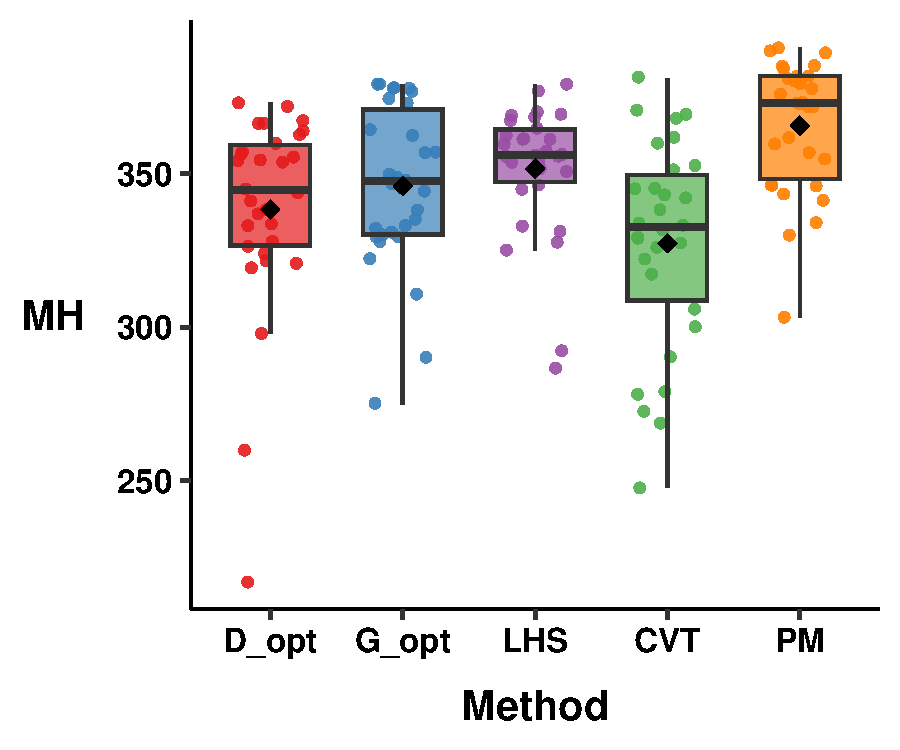
\includegraphics[width=0.45\linewidth]{FIG10a.pdf}}
	\hfill
	\subfigure[QL.]{%
		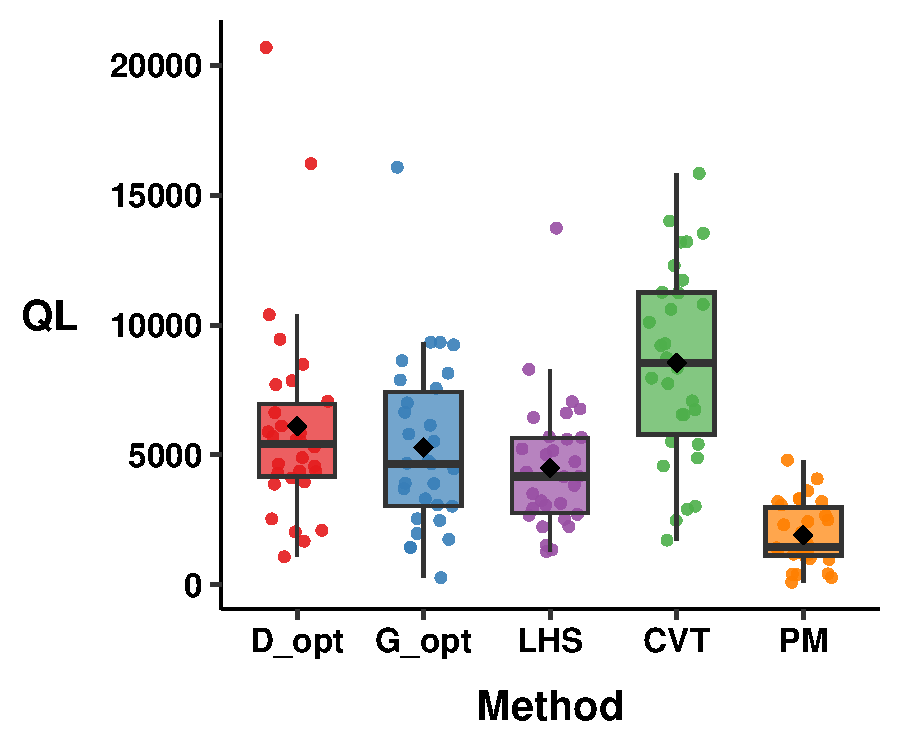
\includegraphics[width=0.45\linewidth]{FIG10b.pdf}}
	
	% --- Second row: Flight trajectories ---
	\vskip\baselineskip
	\subfigure[Flight trajectories.]{%
		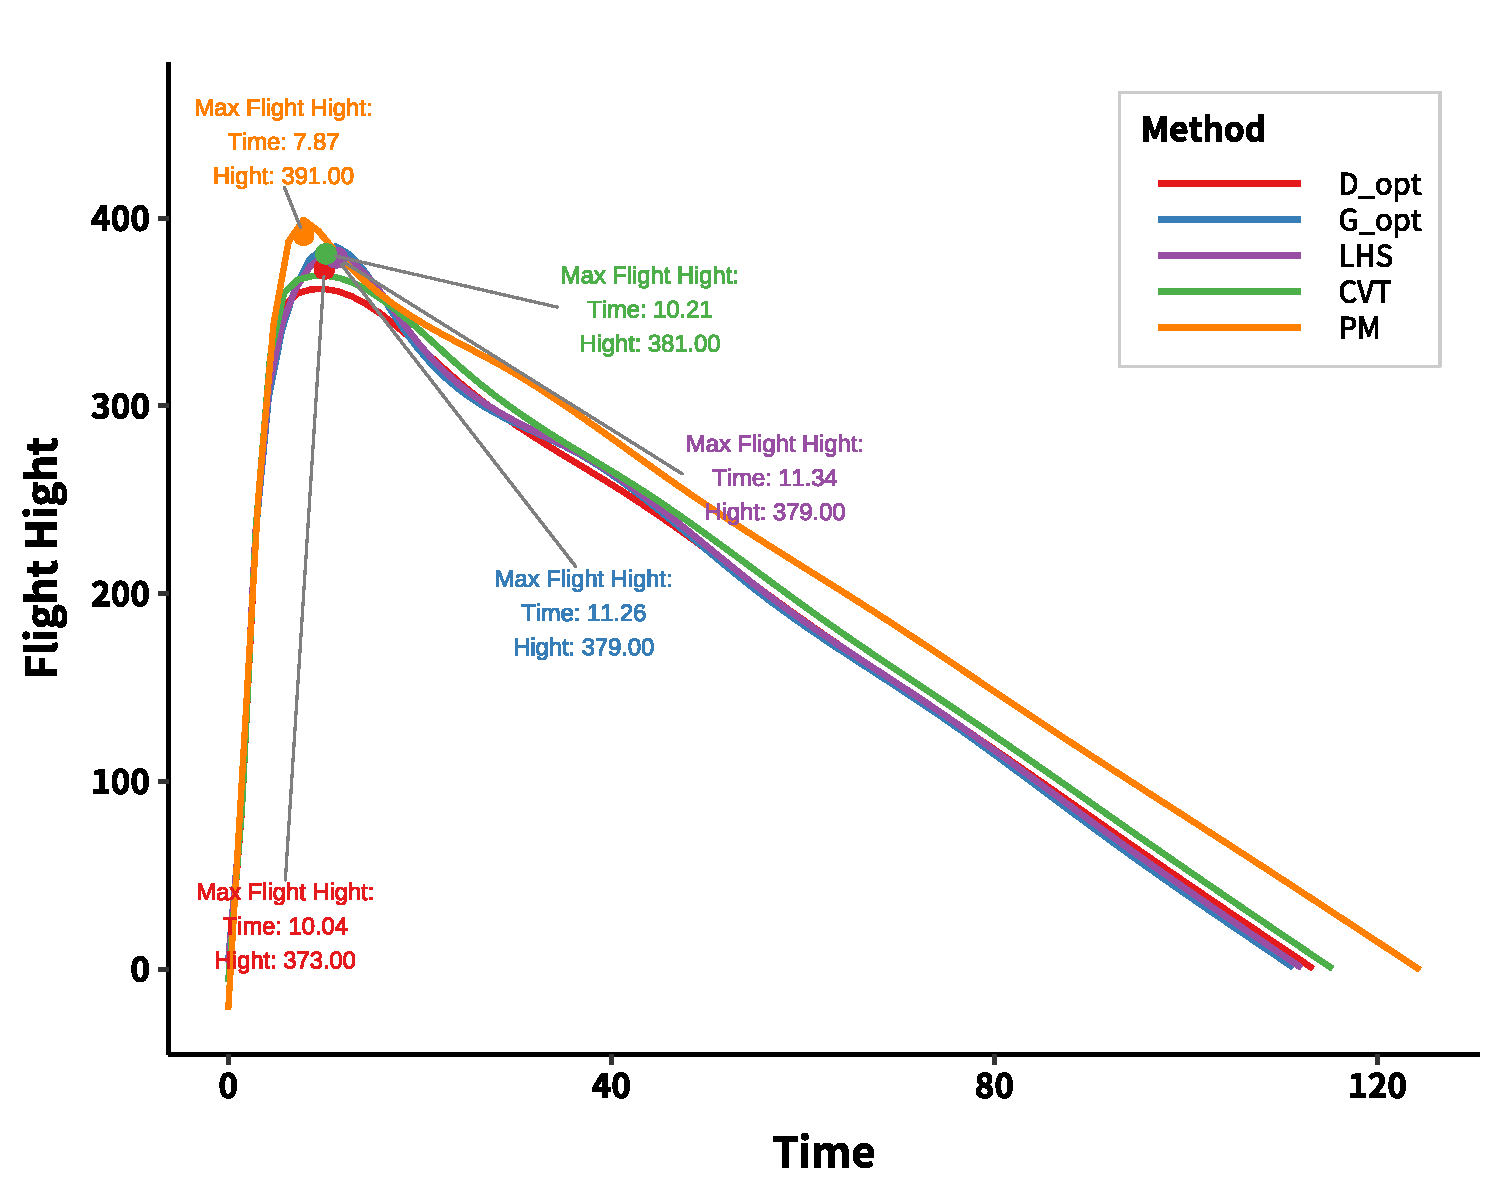
\includegraphics[width=0.45\linewidth]{FIG11.pdf}}
	
	\caption{Optimization results of different methods: 
		(a) MH; (b) QL; (c) Flight trajectories.}
	\label{fig:optimization_results}
\end{figure}


%
%\begin{figure}[h]
%	\centering
%	\subfigure[MH.]{%
%		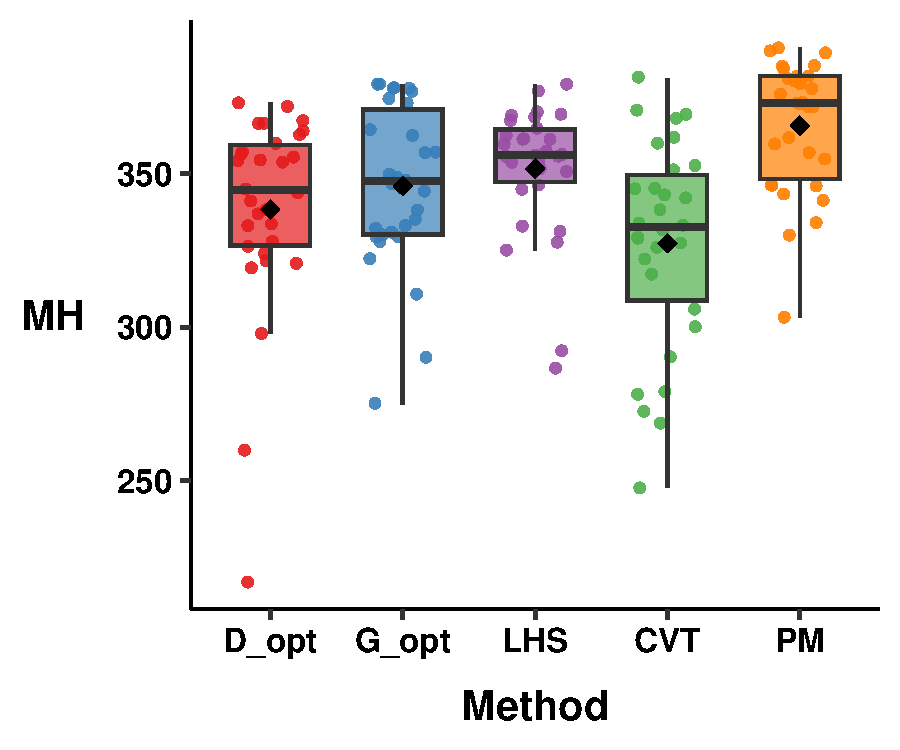
\includegraphics[width=0.45\linewidth]{FIG10a.pdf}}
%	\hfill
%	\subfigure[QL.]{%
%		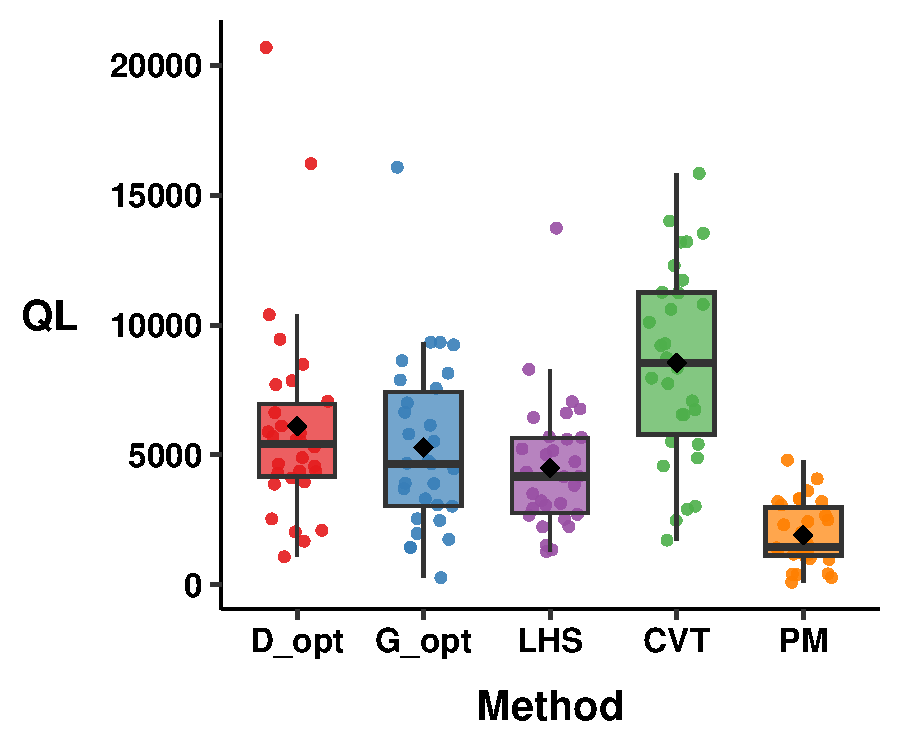
\includegraphics[width=0.45\linewidth]{FIG10b.pdf}}
%	\caption{MH and QL of 30 optimization runs.}
%	\label{fig:mh_ql}
%\end{figure}
%
%
%\begin{figure}[h]
%	\centering
%	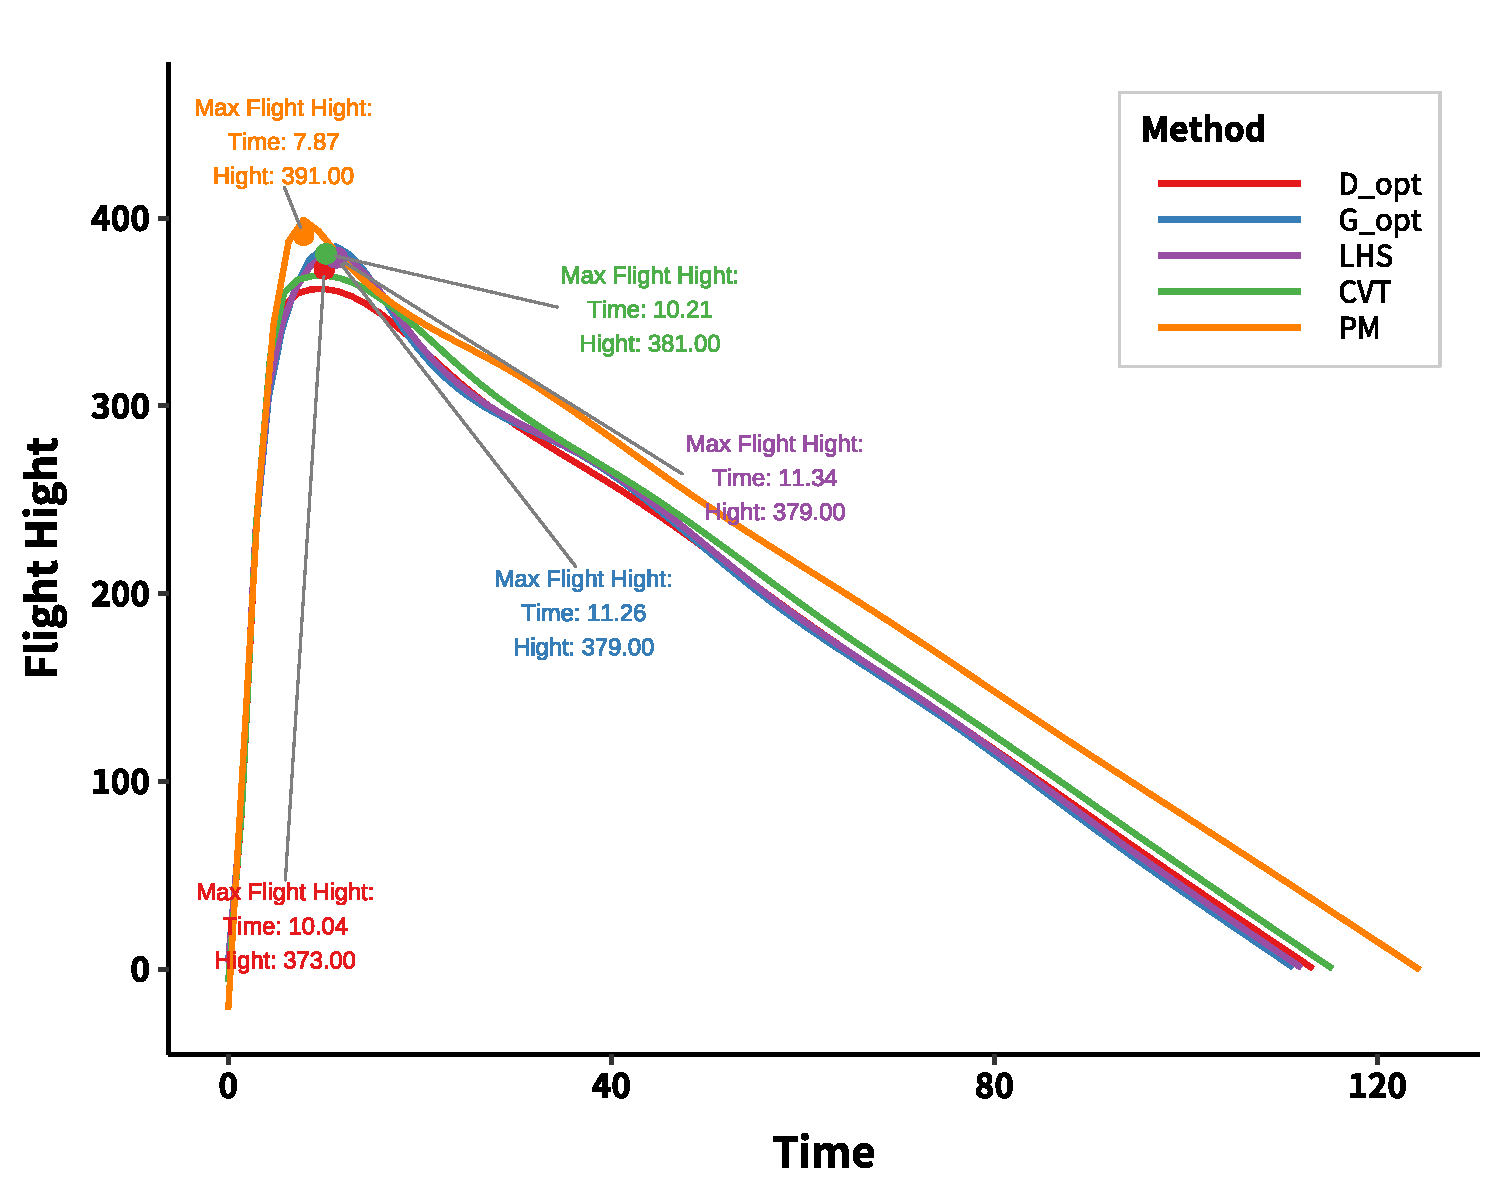
\includegraphics[width=0.5\linewidth]{FIG11.pdf}
%	\caption{Flight trajectories of different methods.}
%	\label{fig:flight_trajectories}
%\end{figure}


Figures 9(a-b) clearly illustrates the performance differences among the methods in terms of MH and QL. Compared with the alternatives, the proposed PM method achieves higher mean and median MH values, with fewer outliers. This indicates greater robustness in the optimization process. For QL, the PM method records both a lower mean and median than the other methods. The results from the 30 experiments are also more tightly clustered, with smaller fluctuations, demonstrating superior optimization performance and stability.

As shown in Table 6, the PM method delivers superior performance across all metrics. Compared with the LHS method, its QL mean decreases from 4496.26 to 1908.09 (a reduction of 57.56\%), and the median decreases by 65.05\%. The maximum and minimum QL values are reduced by 65.06\% and 92.83\%, respectively. For MH, the mean (365.6) and median (373) increase by 3.98\% and 4.78\%, with corresponding maximum and minimum improvements of 3.17\% and 5.57\%. Relative to the CVT method, the PM method achieves reductions in QL mean and median of 22.30\% and 82.95\%, respectively, while the MH mean and minimum increase by 11.69\% and 22.18\%. Compared with the D\-opt method, the QL maximum and mean decrease by 76.81\% and 68.72\%, while the MH mean and median increase by 8.08\% and 8.27\%. In comparison with the G\-opt method, the QL mean, median, and minimum decrease by 63.92\%, 68.76\%, and 66.16\%, respectively, and the MH mean and median increase by 5.69\% and 7.34\%, with maximum and minimum improvements of 3.17\% and 10.18\%.

The results demonstrate that the proposed two-stage active learning algorithm with an attention mechanism can more accurately capture the response surface in the potential optimum region and improve the efficiency of design point utilization. This enhancement significantly increases the effectiveness of the response surface model in robust parameter design and strengthens both the robustness and reliability of the optimal solution.

The optimal solution is determined as the design yielding the highest maximum flight height among the 30 optimization runs. Figure 9(c) presents the MH values and corresponding flight trajectories of the optimal solutions obtained by different methods. Compared with the alternatives, the PM method achieves the best performance in terms of MH, reaching 391 m, which is closer to the target value of 400 m. Regarding flight time, all methods reach the peak altitude in approximately 7.5 s and return to the ground in about 122 s. However, the MH values of the other methods are noticeably lower than that of the PM method. Comparison of the trajectory profiles reveals that, although ascent durations are nearly identical across methods, the PM method provides a more robust optimal solution closer to the target value, thereby improving the efficiency of product quality improvement.

\subsection{Discussion}
This study proposes a two-stage active learning algorithm based on an attention mechanism. Its core lies in constructing an attention model that can dynamically focus on both the potential optimum region and the space-filling performance of design points. This mechanism guides the allocation of newly added design points to the target subregion in a prioritized and balanced manner. As a result, the predictive accuracy within the potential optimum region is substantially improved, thereby enhancing both the robustness and the effectiveness of the optimal solution.

Although the method strengthens local modeling at the cost of a slight reduction in global predictive accuracy, this does not undermine its overall effectiveness. Prioritizing new design points in the potential optimum region markedly improves accuracy in that region and provides a modest positive effect on overall prediction. Because accuracy in the potential optimum region largely determines optimization quality, focusing computational and experimental resources there is essential for effective robust optimization.

Due to the attention-guided iterative updates, computational cost is slightly higher than classical designs (e.g., LHS) but comparable to other active learning methods. The method achieves higher modeling and optimization efficiency for robust parameter design and provides a practical solution for nonstationary response-surface modeling under small-sample conditions.

\section{Conclusion}
To address quality improvement with nonstationary responses under small-sample conditions, an attention-based active learning NSGP modeling and robust optimization framework is proposed. First, a Bayesian hierarchical specification is used to construct the NSGP structure, capturing input-dependent nonstationarity between design variables and output responses. Next, a two-stage attention mechanism is designed to balance quality loss with space-filling, guiding new design points toward the potential optimum region. Finally, the training set and NSGP model are updated, and a quality-loss–based robust optimization model is formulated to obtain the optimal input parameter settings. The key advantage is the two-stage attention-weighted sampling strategy, which efficiently detects the potential optimum region of a nonstationary response, allocates experimental resources to that region, and enhances predictive accuracy in critical areas for optimization. Consequently, design points are used more efficiently and the nonstationary response surface model is more effective. This, in turn, leads to more robust optimization results.

It should be noted that the proposed method adopts a focused attention strategy that prioritizes predictive accuracy in the potential optimum region to improve efficiency in robust parameter design. Global predictive accuracy is not an explicit objective, which may limit applicability to other optimization tasks. Future research is expected to explore multi-level attention mechanisms that jointly consider global and local accuracy, thereby extending the applicability of the proposed approach.



\section*{Disclosure statement}

The authors declare no competing interests.


\section*{Funding}

This work was supported by the National Natural Science Foundation of China [Grant numbers 72301146]; the China Postdoctoral Science Foundation (Grant number 2023M741802, 2024T170430); the China Statistical Science Research Foundation (Grant number 2023LZ010); the Natural Science Foundation of the Jiangsu Higher Education Institutions of China (Grant number 23KJB630012).


\section*{Notes on contributor(s)}
\begin{itemize}
 \item Zebiao Feng received the Ph.D. degree from the School of Economics and Management, Nanjing University of Science and Technology, Nanjing, China, in 2021. He is currently an assistant professor with the School of Management, Nanjing University of Posts and Telecommunications, Nanjing, China. His research interests include quality engineering, computer experiments, and machine learning.

 \item Xu Yang is currently pursuing the M.S. degree in Management Science and Engineering with the School of Management, Nanjing University of Posts and Telecommunications, Nanjing, China. His research interests include quality engineering and machine learning.
 
 \item Jianjun Wang is currently a professor at the School of Economics and Management, Nanjing University of Science and Technology. He received his Ph.D. degree from the School of Economics and Management at Nanjing University of Science and Technology. His research interests include quality engineering, applied statistics, and additive manufacturing.

 \item Weidong Huang is the head and professor of the School of Management at Nanjing University of Posts and Telecommunications. He received his Ph.D. degree in Computer Science and Technology from Nanjing University of Aeronautics and Astronautics. His primary research interests include intelligent optimization, decision making, and emergency management.
\end{itemize}

\section*{Data availability statement}

The authors confirm that the data supporting the findings of this study are available within the article.


\begin{thebibliography}{}

%\bibitem[Alexopoulos et~al.(2022)]{Alexopoulos2022}
%Alexopoulos, K., I. Anagiannis, N. Nikolakis, and G. Chryssolouris. 2022. ``A quantitative approach to resilience in manufacturing systems.'' \emph{International Journal of Production Research} 60(24): 7178--7193.

\bibitem[Alshraideh and del Castillo(2014)]{Alshraideh2014}
Alshraideh, H., and E. del Castillo. 2014. ``Gaussian process modeling and optimization of profile response experiments.'' \emph{Quality and Reliability Engineering International} 30 (4): 449--462.

\bibitem[An et~al.(2020)]{An2020}
An, Y., D. Wang, and X. Zhang. 2020. ``A novel local temperature change detection approach in a 3D thermal field.'' \emph{Quality Technology \& Quantitative Management} 17 (6): 723--737.

\bibitem[Ankenman et~al.(2010)]{Ankenman2010}
Ankenman, B., B. L. Nelson, and J. Staum. 2010. ``Stochastic Kriging for simulation metamodeling.'' \emph{Operations Research} 58 (2): 371--382.

%\bibitem[Aye and Heyns(2018)]{Aye2018}
%Aye, S. A., and P. S. Heyns. 2018. ``Prognostics of slow speed bearings using a composite integrated Gaussian process regression model.'' \emph{International Journal of Production Research} 56 (14): 4860--4873.

\bibitem[Bao et~al.(2016)]{Bao2016}
Bao, L. L., Q. Huang, and K. B. Wang. 2016. ``Robust parameter design for profile quality control.'' \emph{Quality and Reliability Engineering International} 32 (3): 1059--1070.

\bibitem[Barde(2024)]{Barde2024}
Barde, S.. 2024. ``Bayesian estimation of large-scale simulation models with Gaussian process regression surrogates.'' \emph{Computational Statistics \& Data Analysis} 196: 107972.

\bibitem[Box, et~al.(2011)]{Box2011}
Box, S., C. M. Bishop, and H. Hunt. 2011. ``Stochastic six-degree-of-freedom flight simulator for passively controlled high-power rockets.'' \emph{Journal of Aerospace Engineering} 24 (1): 31--45.

\bibitem[Chen and Tuo(2022)]{Chen2022}
Chen, G., and R. Tuo. 2022. ``Projection pursuit Gaussian process regression.'' \emph{IISE Transactions} 55 (9): 901--911.

\bibitem[Chen et~al.(2021)]{Chen2021}
Chen, J. H., L. L. Kang, and G. Lin. 2021. ``Gaussian process assisted active learning of physical laws.'' \emph{Technometrics} 63 (3): 329--342.

\bibitem[Chuang and Wu(2017)]{Chuang2017}
Chuang, C. J., and C. W. Wu. 2017. ``Determining optimal process mean and quality improvement in a profit-maximization supply chain model.'' \emph{Quality Technology \& Quantitative Management} 16 (2): 154--169.


%\bibitem[Cui et~al.(2024)]{Cui2024}
%Cui, F., Z. Jiang, X. Zhou, J. Zheng, and N. Geng. 2024. ``A configuration optimization approach for reconfigurable manufacturing system based on column-generation combined with graph neural network.'' \emph{International Journal of Production Research} 63(3): 970--991.

%\bibitem[Dabbas et~al.(2010)]{Dabbas2010}
%Dabbas, R. M., J. W. Fowler, D. A. Rollier, and D. McCarville. 2010. ``Multiple response optimization using mixture-designed experiments and desirability functions in semiconductor scheduling.'' \emph{International Journal of Production Research} 41 (5): 939--961.

\bibitem[Davis et~al.(2021)]{Davis2021}
Davis, C. B., C. M. Hans, and T. J. Santner. 2021. ``Prediction of non-stationary response functions using a Bayesian composite Gaussian process.'' \emph{Computational Statistics \& Data Analysis} 154: 107083.

\bibitem[Dellino et~al.(2012)]{Dellino2012}
Dellino, G., J. P. C. Kleijnen, and C. Meloni. 2012. ``Robust optimization in simulation: Taguchi and Krige combined.'' \emph{INFORMS Journal on Computing} 24 (3): 471--484.

\bibitem[Ding et~al.(2024)]{Ding2024}
Ding, N., Z. He, S. He, and L. Song. 2024. ``Real-time profile monitoring schemes considering covariates using Gaussian process via sensor data.'' \emph{Quality Technology \& Quantitative Management} 21 (1): 35--53.


\bibitem[Ding et~al.(2004)]{Ding2004}
Ding, R., D. K. J. Lin, and D. Wei. 2004. ``Dual-response surface optimization: a weighted MSE approach.'' \emph{Quality Engineering} 16 (3): 377--385.

%\bibitem[Dong et~al.(2025)]{Dong2025}
%Dong, H., Z. Fan, Q. Wang, W. Zhou, Y. Yu, L. Fu, and J. Li. 2025. ``Modeling, analysis and improvement of production throughput and energy consumption in Li-ion battery manufacturing lines.'' \emph{International Journal of Production Research}: 1--15.

\bibitem[Fan(2000)]{Fan2000}
Fan, S. K. S. 2000. ``A generalized global optimization algorithm for dual response systems.'' \emph{Journal of Quality Technology} 32 (4): 444--456.

\bibitem[Feng et~al.(2021)]{Feng2021}
Feng, Z., J. Wang, Y. Ma, and Y. Tu. 2021. ``Robust parameter design based on Gaussian process with model uncertainty.'' \emph{International Journal of Production Research} 59 (9): 2772--2788.

\bibitem[Feng et~al.(2025)]{Feng2025}
Feng, Z., J. Wang and W. Huang. 2025. ``An active learning multi-objective robust optimization framework via Gaussian process models under uncertainty.'' \emph{Engineering Optimization}: 1-24.


\bibitem[Gelman et~al.(2013)]{Gelman2013}
Gelman, A., H. S. Stern, J. B. Carlin, D. B. Dunson, A. Vehtari, and D. B. Rubin. 2013. \emph{Bayesian Data Analysis}. Chapman and Hall/CRC.

\bibitem[Gnanasambandam et~al.(2024)]{Gnanasambandam2024}
Gnanasambandam, R., B. Shen, A. C. C. Law, C. Dou, and Z. Kong. 2024. ``Deep Gaussian process for enhanced Bayesian optimization and its application in additive manufacturing.'' \emph{IISE Transactions}: 1--14.

\bibitem[Gramacy and Lee(2008)]{Gramacy2008}
Gramacy, R. B., and H. K. H. Lee. 2008. ``Bayesian treed Gaussian process models with an application to computer modeling.'' \emph{Journal of the American Statistical Association} 103 (483): 1119--1130.

\bibitem[Guo et~al.(2023)]{Guo2023}
Guo, B., X. Li, M. Liu, and X. Yang. 2023. ``Construction of orthogonal general sliced Latin hypercube designs.'' \emph{Statistical Papers} 64 (3): 987--1014.

\bibitem[Han et~al.(2023)]{Han2021}
Han, M., Q. Huang, L. Ouyang, and X. Zhao. 2023. ``A kriging-based active learning algorithm for contour estimation of integrated response with noise factors.'' \emph{Engineering with Computers} 39(2): 1341--1362.

\bibitem[Han and Tan(2016)]{Han2016}
Han, M., and M. H. Y. Tan. 2016. ``Integrated parameter and tolerance design with computer experiments.'' \emph{IIE Transactions} 48 (11): 1004--1015.

\bibitem[He et~al.(2021)]{He2021}
He, Z., Y. Gao, L. Qu, and Z. Wang. 2021. ``A nonparametric CUSUM scheme for monitoring multivariate time-between-events-and-amplitude data with application to automobile painting.'' \emph{International Journal of Production Research} 60 (18): 5432--5449.


\bibitem[Heinonen et~al.(2016)]{Heinonen2016}
Heinonen, M., H. Mannerström, J. Rousu, S. Kaski, and H. Lähdesmäki. 2016. ``Non-stationary Gaussian process regression with Hamiltonian Monte Carlo.'' \emph{PMLR}: 732--740.

\bibitem[Hoffman and Gelman(2014)]{Hoffman2014}
Hoffman, M. D., and A. Gelman. 2014. ``The No-U-Turn sampler: adaptively setting path lengths in Hamiltonian Monte Carlo.'' \emph{Journal of Machine Learning Research} 15 (1): 1593--1623.

\bibitem[Huang(2022)]{Huang2022}
Huang, Q.. 2022. ``An impulse response formulation for small-sample learning and control of additive manufacturing quality.'' \emph{IISE Transactions} 55 (9): 926--939.

\bibitem[Jiang and Tan(2021)]{Jiang2021}
Jiang, F., and M. H.-Y. Tan. 2021. ``Shifted log loss Gaussian process model for expected quality loss prediction in robust parameter design.'' \emph{Quality Technology \& Quantitative Management} 18 (5): 527--551.


\bibitem[Kleijnen and Mehdad(2014)]{Kleijnen2014}
Kleijnen, J. P. C., and E. Mehdad. 2014. ``Multivariate versus univariate Kriging metamodels for multi-response simulation models.'' \emph{European Journal of Operational Research} 236 (2): 573--582.

%\bibitem[Komini et~al.(2023)]{Komini2023}
%Komini, L., M. Langelaar, and B. Kriegesmann. 2023. ``Robust topology optimization considering part distortion and process variability in additive manufacturing.'' \emph{Advances in Engineering Software} 186: 103551.

\bibitem[Konomi et~al.(2014)]{Konomi2014}
Konomi, B., G. Karagiannis, A. Sarkar, X. Sun, and G. Lin. 2014. ``Bayesian treed multivariate Gaussian process with adaptive design: Application to a carbon capture unit.'' \emph{Technometrics} 56 (2): 145--158.

%\bibitem[Kontar et~al.(2016)]{Kontar2016}
%Kontar, R., S. Zhou, and J. Horst. 2016. ``Estimation and monitoring of key performance indicators of manufacturing systems using the multi-output Gaussian process.'' \emph{International Journal of Production Research} 55 (8): 2304--2319.

\bibitem[Li et~al.(2025a)]{Li2025}
Li, A., Z. He, Q. Wang, Y. Zhang, and Y. Ma. 2025a. ``A multi-objective evolutionary algorithm with mutual-information-guided improvement phase for feature selection in complex manufacturing processes.'' \emph{European Journal of Operational Research} 323 (3): 952--965.


\bibitem[Li and Ma(2022)]{Li2022}
Li, T., and J. Ma. 2022. ``Attention mechanism based mixture of Gaussian processes.'' \emph{Pattern Recognition Letters} 161: 130--136.

\bibitem[Li et~al.(2025b)]{Liw2025}
Li, W., J. Qin, C. Wu and F. Tsung. 2025b. ``Online monitoring of directed count-weighted network with attributes via the gravity model.''  \emph{Quality Technology \& Quantitative Management}: 1-16.


\bibitem[Li and Zhou(2016)]{Li2016}
Li, Y., and Q. Zhou. 2016. ``Pairwise meta-modeling of multivariate output computer models using nonseparable covariance function.'' \emph{Technometrics} 58 (4): 483--494.

\bibitem[Lichota(2016)]{Lichota2016}
Lichota, P.. 2016. ``Inclusion of the D\_optimality in multisine manoeuvre design for aircraft parameter estimation.'' \emph{Journal of Theoretical and Applied Mechanics} 54 (1): 87--98.

\bibitem[Liu et~al.(2021)]{Liu2021}
Liu, Y., D. Huang, B. Liu, Q. Feng, and B. Cai. 2021. ``Adaptive ranking based ensemble learning of Gaussian process regression models for quality-related variable prediction in process industries.'' \emph{Applied Soft Computing} 101: 107060.

\bibitem[Liu et~al.(2025)]{Liu2025}
Liu, Z., Y. Li, X. Yue, and E. Pan. 2025. ``Latent functional Gaussian process incorporating output spatial correlations.'' \emph{IISE Transactions}: 1--14.

\bibitem[Meng et~al.(2022)]{Meng2022}
Meng, Q., S. Wang, and S. H. Ng. 2022. ``Combined global and local search for optimization with Gaussian process models.'' \emph{INFORMS Journal on Computing} 34 (1): 622--637.

\bibitem[Mustafa et~al.(2024)]{Mustafa2024}
Mustafa, H., C. Bourelly, M. Vitelli, F. Milano, M. Molinara, and L. Ferrigno. 2024. ``SoC estimation on Li-ion batteries: A new EIS-based dataset for data-driven applications.'' \emph{Data Brief} 57: 110947.

\bibitem[Omwando(2024)]{Omwando2024}
Omwando, C. N.. 2024. ``G-criterion for second order rotatable designs constructed using trigonometric transformations.'' \emph{American Journal of Applied Mathematics and Statistics} 12 (3): 70--74.

\bibitem[Ouyang et~al.(2025)]{Ouyang2025}
Ouyang, L., Y. Ling, L. Liu, M. Sun, and M. Wang. 2025. ``Double-robust Bayesian variable selection and model prediction with spherically symmetric error.'' \emph{IISE Transactions}: 1--26.

\bibitem[Ouyang et~al.(2016)]{Ouyang2016}
Ouyang, L., Y. Ma, J. H. Byun, J. Wang, and Y. Tu. 2016. ``An interval approach to robust design with parameter uncertainty.'' \emph{International Journal of Production Research} 54 (11): 3201--3215.

\bibitem[Peterson et~al.(2009)]{Peterson2009}
Peterson, J. J., G. Mir{\'o}-Quesada, and E. del Castillo. 2009. ``A Bayesian reliability approach to multiple response optimization with seemingly unrelated regression models.'' \emph{Quality Technology \& Quantitative Management} 6 (4): 353--369.


\bibitem[Rhode(2020)]{Rhode2020}
Rhode, S.. 2020. ``Non-stationary Gaussian process regression applied in validation of vehicle dynamics models.'' \emph{Engineering Applications of Artificial Intelligence} 93: 103716.

\bibitem[Santner et~al.(2018)]{Santner2018}
Santner, T. J., B. J. Williams, and W. I. Notz. 2018. \emph{Space-filling designs for computer experiments}. New York: Springer.

\bibitem[Sauer et~al.(2022)]{Sauer2022}
Sauer, A., R. B. Gramacy, and D. Higdon. 2022. ``Active learning for deep Gaussian process surrogates.'' \emph{Technometrics} 65 (1): 4--18.

\bibitem[Tan and Wu(2012)]{Tan2012}
Tan, M. H. Y., and C. F. J. Wu. 2012. ``Robust design optimization with quadratic loss derived from Gaussian process models.'' \emph{Technometrics} 54 (1): 51--63.

\bibitem[Vassiliades et~al.(2018)]{Vassiliades2018}
Vassiliades, V., K. Chatzilygeroudis, and J. Mouret. 2018. ``Using centroidal voronoi tessellations to scale up the multidimensional archive of phenotypic elites algorithm.'' \emph{IEEE Transactions on Evolutionary Computation} 22 (4): 623--630.

\bibitem[Wang et~al.(2025)]{Wang2025}
Wang, C., J. Xiao, X. Huang, and J. Xu. 2025. ``RSDS: an efficient adaptive Kriging-based method for structural reliability analysis considering the distance between sample points.'' \emph{Quality Technology \& Quantitative Management}: 1--27.


%\bibitem[Wang et~al.(2023)]{Wang2023}
%Wang, F., A. Wang, T. Tang, and J. Shi. 2023. ``SGL-PCA: Health index construction with sensor sparsity and temporal monotonicity for mixed high-dimensional signals.'' \emph{IEEE Transactions on Automation Science and Engineering} 20 (1): 372--384.

\bibitem[Wang et~al.(2019)]{Wang2019}
Wang, H., J. Yuan, and S. H. Ng. 2019. ``Gaussian process based optimization algorithms with input uncertainty.'' \emph{IISE Transactions} 52 (4): 377--393.

\bibitem[Wang et~al.(2022)]{Wang2022}
Wang, W., X. Yue, B. Haaland, and C. F. J. Wu. 2022. ``Gaussian processes with input location error and applications to the composite parts assembly process.'' \emph{SIAM/ASA Journal on Uncertainty Quantification} 10 (2): 619--650.

%\bibitem[Wang et~al.(2025)]{Wang2025}
%Wang, X., L. J. Hong, Z. Jiang, and H. Shen. 2025. ``Gaussian process-based random search for continuous optimization via simulation.'' \emph{Operations Research} 73 (1): 385--407.

\bibitem[Williams and Rasmussen(2006)]{Williams2006}
Williams, C. K. I., and C. E. Rasmussen. 2006. \emph{Gaussian Processes for Machine Learning}. Cambridge: MIT Press.

\bibitem[Wu and Hamada(2011)]{Wu2011}
Wu, C. F. J., and M. S. Hamada. 2011. \emph{Experiments: Planning, Analysis and Parameter Design Optimization}. New York: John Wiley \& Sons.

\bibitem[Wu et~al.(2020)]{Wu2020}
Wu, C. W., M. H. Shu, and N. Y. Wu. 2020. ``Acceptance sampling schemes for two-parameter Lindley lifetime products under a truncated life test.'' \emph{Quality Technology \& Quantitative Management} 18 (3): 382--395.


%\bibitem[Wu et~al.(2018)]{WuJ2018}
%Wu, J., Y. Yuan, H. Gong, and T. Tseng. 2018. ``Inferring 3D ellipsoids based on cross-sectional images with applications to porosity control of additive manufacturing.'' \emph{IISE Transactions} 50 (7): 570--583.

\bibitem[Xie et~al.(2022)]{Xie2022}
Xie, J., Z. Ma, D. Chang, G. Zhang, and J. Guo. 2022. ``GPCA: A probabilistic framework for Gaussian process embedded channel attention.'' \emph{IEEE Transactions on Pattern Analysis and Machine Intelligence} 44 (11): 8230--8248.

%\bibitem[Xu et~al.(2020)]{Xu2020}
%Xu, T., Y. Liu, L. Tang, and C. Liu. 2020. ``Improvement of Kriging interpolation with learning kernel in environmental variables study.'' \emph{International Journal of Production Research} 60 (4): 1284--1297.

\bibitem[Yu et~al.(2022)]{Yu2022}
Yu, J., S. Li, X. Liu, Y. Gao, S. Wang, and C. Liu. 2022. ``Dynamic convolutional gated recurrent unit attention auto-encoder for feature learning and fault detection in dynamic industrial processes.'' \emph{International Journal of Production Research} 61 (21): 7434--7452.

\bibitem[Zhang et~al.(2024)]{Zhang2024}
Zhang, W., Z. Zhao, H. Xu, X. Li, and Z. Wang. 2024. ``AK-Gibbs: An active learning Kriging model based on Gibbs importance sampling algorithm for small failure probabilities.'' \emph{Computer Methods in Applied Mechanics and Engineering} 426: 116992.

\bibitem[Zhong et~al.(2024)]{Zhong2024}
Zhong, Y., Z. Ling, L. Liu, S. Zhang, and H. Wen. 2024. ``Deep Gaussian attention network for lumber surface defect segmentation.'' \emph{IEEE Transactions on Instrumentation and Measurement} 73: 1--12.

\bibitem[Zhou et~al.(2025)]{Zhou2025}
Zhou, M., R. Zuo, C. Sung, Y. Tong, and X. Wang. 2025. ``Region-optimal Gaussian process surrogate model via Dirichlet process for cold-flow and combustion emulations.'' \emph{Computer Methods in Applied Mechanics and Engineering} 439: 117894.

\end{thebibliography}


\section{Appendices}

\appendix

\section{ }

\begin{table}[h!]
	\centering
	\caption{Maximum RMSE for 10 active learning samples.}
	\begin{tabular}{cccccc}
		\toprule
		Number & D\_opt & G\_opt & LHS & CVT & PM \\
		\midrule
		40 & 0.1976 & 0.1426 & 0.2912 & 0.1105 & 0.1619 \\
		50 & 0.1206 & 0.0990 & 0.0935 & 0.0777 & 0.0840 \\
		60 & 0.0871 & 0.0824 & 0.0679 & 0.1891 & 0.0544 \\
		70 & 0.0826 & 0.0801 & 0.0815 & 0.0784 & 0.0490 \\
		80 & 0.0581 & 0.1178 & 0.0539 & 0.0565 & 0.0440 \\
		90 & 0.0566 & 0.0465 & 0.0409 & 0.0618 & 0.0480 \\
		100 & 0.0313 & 0.0371 & 0.0365 & 0.0510 & 0.0290 \\
		\bottomrule
	\end{tabular}
\end{table}

As shown in Table A1, the PM method consistently achieves superior control over the maximum RMSE, and its advantage becomes increasingly evident as the sample size grows. For example, at 40 total samples, the maximum RMSE is 0.1619, representing a 44.40\% reduction compared with LHS (0.2912). When the sample size increases to 100, the maximum value further decreases to 0.0290—the lowest among all methods—corresponding to a 7.35\% improvement over D\_opt (0.0313) and a 43.14\% improvement over CVT (0.0510). The largest improvement is observed at 60 samples, where PM outperforms CVT by 71.23\%.

\begin{table}[h!]
	\centering
	\caption{Minimum RMSE for 10 active learning samples.}
	\begin{tabular}{cccccc}
		\toprule
		Number & D\_opt & G\_opt & LHS & CVT & PM \\
		\midrule
		40 & 0.0398 & 0.0639 & 0.0265 & 0.0381 & 0.0213 \\
		50 & 0.0143 & 0.0232 & 0.0260 & 0.0167 & 0.0126 \\
		60 & 0.0302 & 0.0064 & 0.0051 & 0.0332 & 0.0210 \\
		70 & 0.0012 & 0.0025 & 0.0234 & 0.0029 & 0.0047 \\
		80 & 0.0191 & 0.0008 & 0.0212 & 0.0208 & 0.0134 \\
		90 & 0.0017 & 0.0204 & 0.0048 & 0.0167 & 0.0122 \\
		100 & 0.0003 & 0.0167 & 0.0067 & 0.0016 & 0.0004 \\
		\bottomrule
	\end{tabular}
\end{table}

As shown in Table A2, the PM method also demonstrates strong competitiveness in terms of minimum RMSE. With 40 samples, PM attains the lowest value of 0.0213, improving by 19.62\% compared with LHS (0.0265) and by 66.67\% compared with G\_opt (0.0639). At 100 samples, the minimum RMSE decreases to 0.0004—comparable to D\_opt (0.0003) but 97.60\% better than G\_opt (0.0167). Although some competing methods slightly outperform PM in certain sample sizes (e.g., 70 and 90), PM maintains a leading position in most cases.

\begin{table}[h!]
	\centering
	\caption{Q1 of RMSE for 10 active learning samples.}
	\begin{tabular}{cccccc}
		\toprule
		Number & D\_opt & G\_opt & LHS & CVT & PM \\
		\midrule
		40 & 0.0665 & 0.0729 & 0.0587 & 0.0490 & 0.0381 \\
		50 & 0.0468 & 0.0542 & 0.0488 & 0.0522 & 0.0322 \\
		60 & 0.0425 & 0.0481 & 0.0371 & 0.0390 & 0.0319 \\
		70 & 0.0380 & 0.0372 & 0.0308 & 0.0298 & 0.0274 \\
		80 & 0.0308 & 0.0315 & 0.0281 & 0.0263 & 0.0212 \\
		90 & 0.0253 & 0.0275 & 0.0231 & 0.0231 & 0.0177 \\
		100 & 0.0210 & 0.0217 & 0.0188 & 0.0211 & 0.0153 \\
		\bottomrule
	\end{tabular}
\end{table}


\begin{table}[h!]
	\centering
	\caption{Q3 of RMSE for 10 active learning samples.}
	\begin{tabular}{cccccc}
		\toprule
		Number & D\_opt & G\_opt & LHS & CVT & PM \\
		\midrule
		40 & 0.1066 & 0.1070 & 0.0908 & 0.0794 & 0.0597 \\
		50 & 0.0741 & 0.0721 & 0.0686 & 0.0661 & 0.0441 \\
		60 & 0.0578 & 0.0604 & 0.0538 & 0.0585 & 0.0420 \\
		70 & 0.0483 & 0.0523 & 0.0442 & 0.0408 & 0.0358 \\
		80 & 0.0415 & 0.0452 & 0.0363 & 0.0394 & 0.0285 \\
		90 & 0.0369 & 0.0357 & 0.0314 & 0.0302 & 0.0238 \\
		100 & 0.0270 & 0.0274 & 0.0268 & 0.0283 & 0.0222 \\
		\bottomrule
	\end{tabular}
\end{table}

To evaluate robustness and consistency, the interquartile range (IQR = Q3 $-$ Q1) derived from Tables A3 and A4 is further analyzed. A smaller IQR indicates a more concentrated and reliable distribution. At 40 samples, PM achieves the smallest IQR of 0.0216 (0.0597 $-$ 0.0381), improving concentration by 28.95\% over CVT (0.0304) and by 46.13\% over D\_opt (0.0401). At 100 samples, the IQR further decreases to 0.0069 (0.0222 $-$ 0.0153), maintaining high robustness. The largest robustness advantage occurs at 50 samples, where the IQR is 0.0119, representing a 56.41\% improvement over D\_opt (0.0273).

\begin{table}[h!]
	\centering
	\caption{Maximum RMSE for 20 active learning samples.}
	\begin{tabular}{cccccc}
		\toprule
		Number & D\_opt & G\_opt & LHS & CVT & PM \\
		\midrule
		40 & 0.3059 & 0.2248 & 0.1732 & 0.1170 & 0.2559 \\
		50 & 0.1864 & 0.0895 & 0.1043 & 0.1075 & 0.2452 \\
		60 & 0.1259 & 0.0999 & 0.0664 & 0.0899 & 0.0404 \\
		70 & 0.0758 & 0.0623 & 0.0574 & 0.0707 & 0.0442 \\
		80 & 0.0750 & 0.0621 & 0.0617 & 0.0670 & 0.0388 \\
		90 & 0.0538 & 0.0481 & 0.0468 & 0.0609 & 0.0512 \\
		100 & 0.0416 & 0.0485 & 0.0462 & 0.0601 & 0.0390 \\
		\bottomrule
	\end{tabular}
\end{table}

As shown in Table A5, the PM method consistently yields the lowest maximum RMSE across all sample sizes. The most significant improvement occurs at 60 samples, where PM reduces the maximum RMSE by 67.91\% compared with D\_opt. Even at 100 samples, PM still achieves a 6.25\% reduction.

\begin{table}[h!]
	\centering
	\caption{Minimum RMSE for 20 active learning samples.}
	\begin{tabular}{cccccc}
		\toprule
		Number & D\_opt & G\_opt & LHS & CVT & PM \\
		\midrule
		40 & 0.0614 & 0.0402 & 0.0287 & 0.0559 & 0.0086 \\
		50 & 0.0336 & 0.0058 & 0.0063 & 0.0364 & 0.0009 \\
		60 & 0.0048 & 0.0232 & 0.0254 & 0.0039 & 0.0081 \\
		70 & 0.0067 & 0.0257 & 0.0129 & 0.0309 & 0.0071 \\
		80 & 0.0003 & 0.0187 & 0.0187 & 0.0044 & 0.0048 \\
		90 & 0.0147 & 0.0144 & 0.0180 & 0.0189 & 0.0002 \\
		100 & 0.0147 & 0.0145 & 0.0073 & 0.0205 & 0.0008 \\
		\bottomrule
	\end{tabular}
\end{table}


Table A6 shows that when the total sample size is 40, PM achieves a minimum RMSE of 0.0086, outperforming all alternatives. The best overall performance is obtained at 50 samples, with a minimum RMSE of 0.0009. The greatest improvement is observed at 90 samples, where PM reduces the minimum RMSE by 98.64\% compared with D\_opt. The smallest gain, at 40 samples, still reaches 69.00\% relative to LHS.

\begin{table}[h!]
	\centering
	\caption{Q1 of RMSE for 20 active learning samples.}
	\begin{tabular}{cccccc}
		\toprule
		Number & D\_opt & G\_opt & LHS & CVT & PM \\
		\midrule
		40 & 0.1081 & 0.0765 & 0.0482 & 0.0741 & 0.0203 \\
		50 & 0.0701 & 0.0449 & 0.0401 & 0.0635 & 0.0185 \\
		60 & 0.0337 & 0.0404 & 0.0291 & 0.0505 & 0.0162 \\
		70 & 0.0341 & 0.0326 & 0.0269 & 0.0431 & 0.0166 \\
		80 & 0.0261 & 0.0308 & 0.0305 & 0.0369 & 0.0154 \\
		90 & 0.0240 & 0.0228 & 0.0214 & 0.0340 & 0.0135 \\
		100 & 0.0232 & 0.0285 & 0.0182 & 0.0266 & 0.0121 \\
		\bottomrule
	\end{tabular}
\end{table}

\begin{table}[h!]
	\centering
	\caption{Q3 of RMSE for 20 active learning samples.}
	\begin{tabular}{cccccc}
		\toprule
		Number & D\_opt & G\_opt & LHS & CVT & PM \\
		\midrule
		40 & 0.1775 & 0.1003 & 0.0861 & 0.0883 & 0.0584 \\
		50 & 0.1237 & 0.0599 & 0.0665 & 0.0782 & 0.0297 \\
		60 & 0.0611 & 0.0553 & 0.0457 & 0.0639 & 0.0242 \\
		70 & 0.0538 & 0.0463 & 0.0438 & 0.0600 & 0.0270 \\
		80 & 0.0418 & 0.0514 & 0.0413 & 0.0482 & 0.0302 \\
		90 & 0.0395 & 0.0346 & 0.0299 & 0.0443 & 0.0230 \\
		100 & 0.0323 & 0.0358 & 0.0271 & 0.0388 & 0.0193 \\
		\bottomrule
	\end{tabular}
\end{table}

Tables A7 and A8 further confirm that PM maintains the smallest interquartile range (IQR = Q3 $-$ Q1) for all sample sizes. This indicates better robustness and concentration. The most pronounced improvement appears at 50 samples, with a 79.10\% gain over D\_opt. Even at 100 samples, PM achieves a 1.37\% improvement compared with G\_opt. These results demonstrate that PM maintains high stability and reliability under varying sample conditions.

\section{ }
\begin{table}[h!]
	\centering
	\caption{Comparison of optimization results with 60 training samples.}
	\label{tab:b1_60}
	\resizebox{\linewidth}{!}{%
		\begin{tabular}{lcccccccccccc}
			\toprule
			\multirow{2}{*}{Method} & \multicolumn{2}{c}{Mean} & \multicolumn{2}{c}{Median} & \multicolumn{2}{c}{Maximum} & \multicolumn{2}{c}{Minimum} & \multicolumn{2}{c}{Q1} & \multicolumn{2}{c}{Q3} \\
			\cmidrule(lr){2-3}\cmidrule(lr){4-5}\cmidrule(lr){6-7}\cmidrule(lr){8-9}\cmidrule(lr){10-11}\cmidrule(lr){12-13}
			& MH & QL & MH & QL & MH & QL & MH & QL & MH & QL & MH & QL \\
			\midrule
			PM     & 365.83 & 2930.53 & 371.50 & 3013.73 & 392.00 & 6720.97 & 300.00 & 1018.22 & 350.00 & 2160.40 & 383.00 & 3456.65 \\
			LHS    & 351.87 & 5784.58 & 353.50 & 5342.49 & 377.00 & 9498.79 & 320.00 & 2690.94 & 347.00 & 4459.98 & 359.00 & 7648.59 \\
			CVT    & 325.97 & 8622.45 & 339.50 & 7396.28 & 365.00 & 21212.57 & 246.00 &  777.46 & 307.00 & 6151.12 & 353.50 & 10521.37 \\
			D\_opt & 328.20 & 7570.85 & 340.50 & 6076.41 & 388.00 & 19800.33 & 239.00 & 1474.00 & 301.25 & 4308.73 & 357.50 & 9276.37 \\
			G\_opt & 334.27 & 7235.88 & 338.00 & 6161.14 & 391.00 & 17281.67 & 251.00 & 1879.86 & 319.00 & 4146.96 & 356.25 & 9606.40 \\
			\bottomrule
		\end{tabular}%
	}
\end{table}

As shown in Table B1, the PM method consistently outperforms other approaches with 60 training samples. Compared with LHS, the PM method reduces the QL mean from 5784.58 to 2930.53, achieving a 49.34\% decrease. The median and minimum QL values are also reduced by 43.59\% and 62.16\%, respectively. For the MH metric, the PM method improves the mean, median, and maximum by 3.97\%, 5.09\%, and 3.98\%. Relative to CVT, PM shows even stronger performance. It reduces the QL mean by 66.01\%, the median by 59.25\%, and the maximum by 68.32\%. Meanwhile, MH performance improves by 12.23\% in the mean and 21.95\% in the minimum. When compared with D\_opt, PM lowers the QL mean by 61.29\% and the maximum by 66.06\%. It also increases the MH mean by 11.47\% and the median by 9.10\%. Compared with G\_opt, the QL mean, median, maximum, and minimum are reduced by 59.50\%, 51.08\%, 61.10\%, and 45.84\%, respectively. Additionally, the MH mean and median are improved by 9.44\% and 9.91\%, while the minimum increases by 19.52\%.

\begin{table}[h!]
	\centering
	\caption{Comparison of optimization results with 70 training samples.}
	\label{tab:b2_70}
	\resizebox{\linewidth}{!}{%
		\begin{tabular}{lcccccccccccc}
			\toprule
			\multirow{2}{*}{Method} & \multicolumn{2}{c}{Mean} & \multicolumn{2}{c}{Median} & \multicolumn{2}{c}{Maximum} & \multicolumn{2}{c}{Minimum} & \multicolumn{2}{c}{Q1} & \multicolumn{2}{c}{Q3} \\
			\cmidrule(lr){2-3}\cmidrule(lr){4-5}\cmidrule(lr){6-7}\cmidrule(lr){8-9}\cmidrule(lr){10-11}\cmidrule(lr){12-13}
			& MH & QL & MH & QL & MH & QL & MH & QL & MH & QL & MH & QL \\
			\midrule
			PM     & 369.53 & 3527.62 & 374.50 & 2863.82 & 392.00 & 8610.52 & 318.00 & 1854.14 & 360.50 & 2516.13 & 380.50 & 4044.50 \\
			LHS    & 346.00 & 7056.32 & 352.00 & 6489.23 & 384.00 & 19136.57 & 242.00 & 1914.78 & 334.50 & 4823.50 & 362.25 & 8758.49 \\
			CVT    & 336.07 & 8476.93 & 341.50 & 7220.50 & 385.00 & 26473.52 & 261.00 & 2497.03 & 327.50 & 5729.68 & 351.00 & 9735.58 \\
			D\_opt & 335.33 & 8640.93 & 338.50 & 7532.22 & 374.00 & 25676.47 & 233.00 & 3308.62 & 323.75 & 4919.09 & 356.25 & 10550.84 \\
			G\_opt & 334.07 & 7835.69 & 335.00 & 5989.16 & 387.00 & 18779.07 & 275.00 & 2748.34 & 313.75 & 4785.09 & 361.00 & 10509.83 \\
			\bottomrule
		\end{tabular}%
	}
\end{table}

As shown in Table B2, with 70 training samples, the PM method consistently outperforms all other methods across key indicators. Compared with LHS, PM reduces the QL mean from 7056.32 to 3527.62, achieving a 50.00\% reduction. The median and maximum QL values are reduced by 55.88\% and 55.00\%, respectively. Meanwhile, MH improves by 6.80\% in the mean, 6.39\% in the median, and 31.40\% in the minimum. Against CVT, PM lowers the QL mean by 58.38\% and the maximum by 67.48\%. The MH mean increases by 9.96\%, while the minimum rises by 21.84\%. Compared with D\_opt, PM achieves a 59.18\% reduction in QL mean and a 66.46\% drop in the maximum. At the same time, MH improves by 10.20\% in the mean and 36.48\% in the minimum. Relative to G\_opt, QL values are significantly lower. The mean and median are reduced by 54.98\% and 52.18\%, respectively. In terms of MH, the mean increases by 10.61\%, the median by 11.79\%, and the minimum by 15.64\%.

\begin{table}[h!]
	\centering
	\caption{Comparison of optimization results with 80 training samples.}
	\label{tab:b3_80}
	\resizebox{\linewidth}{!}{%
		\begin{tabular}{lcccccccccccc}
			\toprule
			\multirow{2}{*}{Method} & \multicolumn{2}{c}{Mean} & \multicolumn{2}{c}{Median} & \multicolumn{2}{c}{Maximum} & \multicolumn{2}{c}{Minimum} & \multicolumn{2}{c}{Q1} & \multicolumn{2}{c}{Q3} \\
			\cmidrule(lr){2-3}\cmidrule(lr){4-5}\cmidrule(lr){6-7}\cmidrule(lr){8-9}\cmidrule(lr){10-11}\cmidrule(lr){12-13}
			& MH & QL & MH & QL & MH & QL & MH & QL & MH & QL & MH & QL \\
			\midrule
			PM     & 366.60 & 5597.53 & 372.50 & 4794.50 & 392.00 & 14924.09 & 319.00 & 2131.16 & 356.00 & 3481.38 & 378.00 & 5943.41 \\
			LHS    & 350.67 & 8907.73 & 356.00 & 8332.60 & 384.00 & 21441.47 & 272.00 & 3271.37 & 343.00 & 6424.00 & 361.00 & 10717.41 \\
			CVT    & 335.57 & 10070.66 & 336.50 & 9343.45 & 371.00 & 18541.11 & 277.00 & 2641.21 & 323.50 & 7482.70 & 352.00 & 12569.66 \\
			D\_opt & 319.40 & 12093.48 & 323.00 & 10690.87 & 372.00 & 22646.91 & 252.00 & 3865.38 & 305.00 & 8724.00 & 349.75 & 16243.79 \\
			G\_opt & 334.57 & 9588.88 & 342.00 & 8141.33 & 389.00 & 21515.31 & 235.00 & 3256.61 & 322.75 & 6710.74 & 359.75 & 12136.71 \\
			\bottomrule
		\end{tabular}%
	}
\end{table}

As shown in Table B3, with 80 training samples, the PM method continues to outperform all competing methods. Compared with LHS, PM reduces the QL mean from 8907.73 to 5597.53, representing a 37.16\% reduction. The median QL is also reduced by 42.46\%. In terms of MH, the mean and median increase by 4.54\% and 4.63\%, respectively, while the minimum rises by 17.28\%. Relative to CVT, PM lowers the QL mean by 44.42\% and the median by 48.69\%. It also improves the MH mean by 9.25\% and the minimum by 15.16\%. Compared with D\_opt, PM achieves a 53.72\% reduction in QL mean. The MH mean and median increase by 14.78\% and 15.32\%, respectively, and the minimum improves by 26.59\%. Against G\_opt, PM achieves a 41.62\% reduction in QL mean and a 41.11\% decrease in median. MH performance also improves, with the mean and median increasing by 9.57\% and 8.92\%, respectively, and the minimum rising by 35.74\%.











\end{document}
